% concatenated from arxiv_submission.tex
\documentclass[12pt, reqno]{amsart}
\usepackage[utf8]{inputenc}
\usepackage[english]{babel}

% General Packages
\usepackage{ifthen}
\usepackage{microtype}
\usepackage[dvipsnames]{xcolor}
\usepackage{comment}
\usepackage{blkarray}
\usepackage{fullpage}
\usepackage{mathtools}
\usepackage{xfrac}
\usepackage{shuffle}
\usepackage{centernot}
\usepackage{enumitem}
%\usepackage{MnSymbol}
\usepackage{mathdots}
\usepackage{multirow}
\usepackage{amssymb}
\usepackage{soul}
\usepackage{booktabs}
\usepackage{diagbox}
\usepackage{multicol}
\setlength{\columnsep}{-.5cm}
\setlength{\multicolsep}{-1.0pt plus 0.0pt minus 1.5pt}% Sort and compress citations
\usepackage[noadjust]{cite}

\usepackage{amsmath}

\newlist{paraenum}{enumerate}{1}
\setlist[paraenum]{wide, label=(\arabic*)}

% Remove indentation from addresses at the end of the document.
% https://tex.stackexchange.com/a/560609
\makeatletter
\patchcmd{\@setaddresses}{\indent}{\noindent}{}{}
\patchcmd{\@setaddresses}{\indent}{\noindent}{}{}
\patchcmd{\@setaddresses}{\indent}{\noindent}{}{}
\patchcmd{\@setaddresses}{\indent}{\noindent}{}{}
\makeatother

% Figure formatting
\usepackage{caption}
\usepackage{subcaption}
\captionsetup[subfigure]{labelfont=rm}

% tikz
\usepackage{tikz}    
\usetikzlibrary{cd}
\usetikzlibrary{backgrounds}
\usetikzlibrary{shapes}
\usetikzlibrary{arrows}
\usetikzlibrary{positioning}
\usetikzlibrary{calc}
\usetikzlibrary{quotes}
\usetikzlibrary{fit}
\usetikzlibrary{decorations.pathreplacing}



% reference formatting
\usepackage[pdftex]{hyperref}
\hypersetup{
    colorlinks=true,
    linkcolor={magenta},
    citecolor={blue},
    urlcolor={blue}
    %allbordercolors={1 0 0}
}
\usepackage[capitalise]{cleveref}



% Theorem styles
\numberwithin{equation}{section}
\theoremstyle{plain}
\newtheorem{theorem}{Theorem}[section]
\newtheorem{conjecture}[theorem]{Conjecture}
\newtheorem{corollary}[theorem]{Corollary}
\newtheorem{lemma}[theorem]{Lemma}
\newtheorem{proposition}[theorem]{Proposition}
\newtheorem{problem}[theorem]{Problem}
\newtheorem{question}[theorem]{Question}

\theoremstyle{definition}
\newtheorem{remark}[theorem]{Remark}
\newtheorem{examplex}[theorem]{Example}
\newenvironment{example}
  {\pushQED{\qed}\renewcommand{\qedsymbol}{$\triangle$}\examplex}
  {\popQED\endexamplex}
\newtheorem{ques}[theorem]{Question}
\newtheorem{definition}[theorem]{Definition}
\newtheorem{observation}[theorem]{Observation}
\newtheorem{claim}[theorem]{Claim}
\newtheorem{fact}[theorem]{Fact}
\newtheorem{construction}[theorem]{Construction}
\newtheorem{convention}[theorem]{Convention}

%% Sets of numbers
\newcommand{\cc}{\mathbb{C}}
\newcommand{\rr}{\mathbb{R}}
\newcommand{\qq}{\mathbb{Q}}
\newcommand{\zz}{\mathbb{Z}}
\newcommand{\nn}{\mathbb{N}}
\newcommand{\kk}{\mathbb{K}}
\newcommand{\pp}{\mathbb{P}}

% Caligraphics
\newcommand{\cd}{\mathcal{D}}
\newcommand{\cs}{\mathcal{S}}
\newcommand{\cm}{\mathcal{M}}
\newcommand{\cn}{\mathcal{N}}
\newcommand{\ct}{\mathcal{T}}
\newcommand{\cg}{\mathcal{G}}
\newcommand{\ci}{\mathcal{I}}
\newcommand{\cv}{\mathcal{V}}
\newcommand{\cz}{\mathcal{Z}}
\newcommand{\cb}{\mathcal{B}}


%%%%%%%%%%%%%%%%%%%%   Math operators    %%%%%%%%%%%%%%%%%%%%
\DeclareMathOperator{\codim}{codim}
\DeclareMathOperator{\df}{def}
\DeclareMathOperator{\diam}{diam} 
\DeclareMathOperator{\dir}{dir}
\DeclareMathOperator{\girth}{girth} 
\DeclareMathOperator{\Inv}{Inv} 
\DeclareMathOperator{\length}{length}
\DeclareMathOperator{\nul}{nul}
\DeclareMathOperator{\rad}{rad}
\DeclareMathOperator{\jac}{Jac}
\DeclareMathOperator{\rank}{rank}
\DeclareMathOperator{\rt}{root}
\DeclareMathOperator{\sign}{sign} 
\DeclareMathOperator{\tail}{tail}
\DeclareMathOperator{\ter}{ter}
\DeclareMathOperator{\val}{val}
\DeclareMathOperator{\wt}{wt}
\DeclareMathOperator{\Hom}{Hom}
\DeclareMathOperator{\interior}{int}
\DeclareMathOperator{\image}{image}
\DeclareMathOperator{\perm}{Perm}
\DeclareMathOperator{\var}{Var}
\DeclareMathOperator{\tr}{tr}
\DeclareMathOperator{\adj}{adj}
\DeclareMathOperator{\Adj}{Adj}
%\DeclareMathOperator{\span}{span}

% Paper-specific commands
\newcommand{\fraks}{\frak{S}}
\DeclareMathOperator{\lift}{lift}
\newcommand{\monbar}{\overline{\mathcal{M}}_{0, n}}
\newcommand{\pt}{\mathrm{PT}}
\newcommand{\lc}{\mathrm{LC}}
\newcommand{\inv}{\mathrm{inv}}
\newcommand{\gr}{\mathrm{Gr}}
\DeclareRobustCommand{\abinom}{\genfrac{\langle}{\rangle}{0pt}{}}

% Editing colors
\definecolor{benpurple}{RGB}{180, 0, 240}
\newcommand\dm[1]{{\color{red}(Dmitrii: #1)}}
\newcommand\bh[1]{{\color{benpurple}(Ben: #1)}}
\newcommand{\tocite}{\textcolor{benpurple}{CITE}}


\title{Parke--Taylor Varieties}


\author{Benjamin Hollering}
\address{Max Planck Institute for Mathematics in the Sciences, Inselstr. 22, 04103 Leipzig, Germany}
\email{benjamin.hollering@mis.mpg.de}


\author{Dmitrii Pavlov}
\address{Technische Universit\"at Dresden, Zellescher Weg 12--14, 01069 Dresden, Germany}
\email{dmitrii.pavlov@mis.mpg.de}

\date{}

\begin{document}


\begin{abstract}
Parke--Taylor functions are certain rational functions on the Grassmannian of lines encoding MHV amplitudes in particle physics. For $n$ particles there are $n!$ Parke--Taylor functions, corresponding to all orderings of the particles. Linear relations between these functions have been extensively studied in the last years. We here describe all non-linear polynomial relations between these functions in a simple combinatorial way and study the variety parametrized by them, called the Parke--Taylor variety. We show that the Parke--Taylor variety is linearly isomorphic to the log canonical embedding of the moduli space $\overline{\mathcal{M}}_{0,n}$ due to Keel and Tevelev, and that the intersection with the algebraic torus recovers the open part, $\mathcal{M}_{0,n}$. We give an explicit description of this isomorphism. Unlike the log canonical embedding, this Parke--Taylor embedding respects the symmetry of the $n$ marked points and is constructed in a single-step procedure, avoiding the intermediate embedding into a product of projective spaces.
\end{abstract}

\maketitle

\section{Introduction}
A Parke--Taylor function is a rational function of the form 
$$f_\sigma = \dfrac{1}{\prod\limits_{i=1}^n p_{\sigma_i\sigma_{i+1}}},$$
where $p_{ij}$ are the Pl\"ucker coordinates on the Grassmannian of lines $\mathrm{Gr}(2,n)$, $\sigma$ is a permutation on $[n]=\{1,\ldots,n\}$ and the indices are understood modulo $n$. In particle physics, Parke--Taylor functions are key components of the Parke--Taylor formula \cite{parke1986amplitude}, a strikingly simple expression for \emph{maximally helicity violating (MHV)} amplitudes. In this context $n$ is the number of particles in a scattering process. They also arise in numerous related contexts in scattering amplitudes, such as the CHY formalism \cite{cachazo2014scattering}, the momentum amplituhedron \cite{damgaard2021kleiss}, and CEGM amplitudes \cite{cachazo2024color} to name a few. 

For a scattering process of $n$ particles there are $n!$ Parke--Taylor functions, one for each ordering of the particles. Linear relations between these $n!$ functions, also called linear \emph{Parke--Taylor identities}, are also of interest in the aforementioned contexts, and have been studied in both the physics \cite{cachazo2019delta,AH2015nonplanar,frost2021lie,cachazo2024color,damgaard2021kleiss} and mathematics \cite{parisi2024magic} literature. However, to the best of our knowledge, there is no systematic description of \emph{polynomial} relations between the $n$-point Parke--Taylor functions. The main goal of this paper is to present such a description. 

More precisely, we are interested in the polynomial relations that are not implied by the linear Parke--Taylor identities. It is well-known that the $(n-2)!$ Parke--Taylor functions $f_\sigma$ with $\sigma_1=1$ and $\sigma_2=2$ form a basis of the $\mathbb{C}$-linear space spanned by all $n!$ Parke--Taylor functions. This is ensured by the Kleiss--Kuijf relations (see e.g. \cite[Lemma 2.2]{frost2021lie} or \cite{damgaard2021kleiss}). We will therefore only describe relations between such functions. The methods we use come from computational (nonlinear \cite{michalek2021invitation}) algebra. We define an \emph{algebraic variety} in $\mathbb{P}^{(n-2)!-1}$ \emph{parametrized} by the Parke--Taylor functions. That is, we consider the image of the map $\mathrm{Gr}(2,n)\dashrightarrow \mathbb{P}^{(n-2)!-1}$ given by these functions. We call this image the \emph{open Parke--Taylor variety} and denote it by $\mathrm{PT}^\circ_n$. Its Zariski closure (that is, the smallest projective variety containing it) is then called the \emph{Parke--Taylor variety} and is denoted by  $\mathrm{PT}_n$. We then \emph{implicitize} these varieties, that is, find their defining equations. For details on the definition of Parke--Taylor varieties, see Section \ref{sec:prelim}.

While our study of Parke--Taylor varieties is primarily motivated by physics, they turn out to be quite interesting objects from a purely mathematical point of view. The ambient space of the Parke--Taylor variety $\mathrm{PT}_n$ is the projective space $\mathbb{P}^{(n-2)!-1}$. This is also the ambient space of the log canonical embedding of the moduli space of stable $n$-pointed rational curves $\overline{\mathcal{M}}_{0,n}$ constructed by Keel and Tevelev \cite{keel2009equations}. The moduli space $\overline{\mathcal{M}}_{0,n}$ is a compactification of $\mathcal{M}_{0,n}$, the moduli space of $n$ marked points on $\mathbb{P}^1$, known as the \emph{Deligne--Knudsen--Mumford} compactification.
The log canonical embedding is arguably the most standard way of realizing $\overline{\mathcal{M}}_{0,n}$ as a subvariety in the projective space. 
In Theorem \ref{thm:log-canon-Parke--Taylor} we show that the Parke--Taylor variety $\mathrm{PT}_n$ is linearly isomoprhic to the log canonical embedding $\mathrm{LC}_n$ of $\overline{\mathcal{M}}_{0,n}$, and that the linear isomorphism has an elegant, explicit combinatorial description.
We note that the construction of the log canonical embedding involves iteratively applying Kapranov's map $\monbar\to\overline{\mathcal{M}}_{0,n-1}$ \cite{kapranov1993veronese} obtained by forgetting one marked point and stabilizing the resulting $n-1$-pointed curve. This breaks the symmetry of the $n$ marked points on a stable curve by forgetting them one at a time. 
Our construction is on the contrary almost completely symmetric: the only choice we make is that of the two fixed points $1$ and $2$. 
This can also be avoided by considering the variety in $\mathbb{P}^{n!-1}$ parametrized by all $n!$ Parke--Taylor functions, which makes the Parke--Taylor variety invariant under the action of $S_n$ on the indices of the Parke--Taylor functions.
Another important feature of this \emph{Parke--Taylor embedding} is that the open Parke--Taylor variety recovers the moduli space $\mathcal{M}_{0,n}$ (Theorem \ref{thm:PTM0n}). 

The task of describing the nonlinear Park--Taylor identities is therefore the task of describing the equations of a specific projective embedding of $\monbar$. 
For various embeddings of this moduli space, this question has been extensively studied in the literature, and we now give a brief overview of the results.
For the log canonical embedding, Monin and Rana \cite{monin2017equations} conjectured a set of equations that define it scheme-theoretically, and verified this conjecture for $n\leq 8$.
This conjecture was proven for all $n$ by Gillespie, Griffin and Levinson in \cite{gillespie2022proof}. 
In \cite{maclagan2010chow}, Gibney and Maclagan embed $\monbar$ into a (rather high-dimensional) toric variety and describe the ideal of this embedding up to saturation. 
As noted in \cite[Section 1]{monin2017equations}, this embedding is different from the log canonical embedding. 
Both these embeddings stem from the fact that $\monbar$ is a Chow quotient of the Grassmannian of lines $\mathrm{Gr}(2,n)$ \cite{kapranov1993chow}. 
Finally, in \cite{vakil2009equations} the authors study a rather general question of determining the equations for the moduli space of $n$ points on a line in the presence of weights, and their starting point is representing the moduli space as a GIT quotient of a product of projective lines.

The explicit linear isomorphism between the Parke--Taylor variety $\mathrm{PT}_n$ and the log canonical embedding $\mathrm{LC}_n$ of $\monbar$, in combination with the results of \cite{monin2017equations, gillespie2022proof}, suggests one way of describing the defining equations of $\mathrm{PT}_n$. One can just take the equations of $\mathrm{LC}_n$ and apply the linear isomorphism from Theorem \ref{thm:log-canon-Parke--Taylor} to them. This description, however, is not particularly explicit. The log canonical embedding is the composition of an embedding $\monbar \hookrightarrow \mathbb{P}^1\times\ldots\times\mathbb{P}^{n-3}$ and the Segre embedding $\mathbb{P}^1\times\ldots\times\mathbb{P}^{n-3}\hookrightarrow \mathbb{P}^{(n-2)!-1}$, and \cite{monin2017equations, gillespie2022proof} concentrate on describing the equations of $\monbar$ in the product of projective spaces, before the Segre embedding. The work of Keel and Tevelev \cite{keel2009equations} provides a way to transform these into equations in $\mathbb{P}^{(n-2)!-1}$, which is compactly described in \cite[Section 1]{monin2017equations}. However, this transformation is not entirely trivial: for instance, the equations of Monin and Rana are cubic; however, the ideal in $\mathbb{P}^{(n-2)!-1}$ is quadratically generated \cite[Theorem 8.6]{keel2009equations}. For this reason, we opt for presenting a more explicit description of the ideal of $\mathrm{PT}_n$. Here we use the fact that the Parke--Taylor embedding is defined in a more straightforward way than the log canonical embedding (and the embeddings of \cite{maclagan2010chow} and \cite{vakil2009equations}): it is the closure of the image of a single rational (essentially, monomial) map from $\mathrm{Gr}(2,n)$ directly into $\mathbb{P}^{(n-2)!-1}$.

Our description gives the ideal of $\mathrm{PT}_n$ up to saturation by the product of the variables. It is based on the following observation: the map $\varphi_n:\mathrm{Gr}(2,n)\dashrightarrow \mathbb{P}^{(n-2)!-1}$ defining $\mathrm{PT}_n$ is a monomial map in the inverses $\frac{1}{p_{ij}}$ of the Pl\"ucker variables. This map can be extended to the whole Pl\"ucker space $\mathbb{P}^{\binom{n}{2}-1}$. The closure of the image of this extended map is a toric variety, which we denote by $T_n$, and its defining equations are binomial. We then have a natural inclusion $\mathrm{PT}_n\subset T_n$. The equations of $\mathrm{PT}_n$ therefore come in two flavors: those of the first type are the binomial equations of $T_n$, and those of the second type are \emph{lifts} of the Pl\"ucker relations defining $\mathrm{Gr}(2,n)$ inside $\mathbb{P}^{\binom{n}{2}-1}$. We describe these two types of equations in Sections \ref{sec:toric} and \ref{sec:idealPT} respectively.


Finally, we note that this topic also has an algebraic statistics flavor. The real positive points of the Parke--Taylor variety $\mathrm{PT}_n$ can be regarded as a statistical model for ranked data as considered in \cite{sturmfels2012statistical}. We note that such a \emph{Parke--Taylor model} is distinct from the three toric models studied in \cite{sturmfels2012statistical} for all $n \geq 5$. In particular, the toric Parke--Taylor model is lower-dimensional than the other models and thus its ideal is generated by more polynomials, which we conjecture have unbounded degree as $n$ grows. 

The remainder of this article is organized as follows. In Section \ref{sec:prelim} we give some basic notions of computational algebra and algebaric geometry and define Parke--Taylor varieties.
Although the notions we describe are quite basic from the point of view of an algebraist, we find it useful to present them here to make the article accessible to a broad range of readers, including those from the physics community.
In Section \ref{sec:PTM0n} we connect Parke--Taylor varieties to moduli spaces. Theorem \ref{thm:PTM0n} establishes an isomorphism between the open Parke--Taylor variety $\mathrm{PT}_n^\circ$ and $\mathcal{M}_{0,n}$, and Theorem \ref{thm:log-canon-Parke--Taylor} gives a linear isomorphism between $\mathrm{PT}_n$ and the log canonical embedding $\mathrm{LC}_n$ of $\monbar$. We use this to establish the degree of $\mathrm{PT}_n$ and show that its ideal is generated by quadrics.
In Section \ref{sec:toric} we take a first step towards describing the equations that cut out $\mathrm{PT}_n$. 
More precisely, we describe all \emph{binomial} relations that hold on this variety. 
They cut out the \emph{toric Parke--Taylor variety} $T_n$ which contains $\mathrm{PT}_n$. 
These binomial relations admit a particularly simple combinatorial description, which we present in Proposition \ref{prop:toric-gens-via-adjs}. 
In Theorem \ref{thm:toricquadratics} we describe a set of \emph{quadratic} binomials, which we conjecture is enough to generate the ideal of $T_n$ for $n\geq 7$ up to saturation by the product of the variables. 
We verify this for $n\leq 9$.
Finally, in Section \ref{sec:idealPT} we describe the full ideal of the Parke--Taylor variety. 
In Theorem \ref{thm:fullideal} we show that to generate the ideal of $\mathrm{PT}_n$ it is enough to know all the binomial relations (that is, the ideal of $T_n$) and the \emph{lift} of an $n-3$-dimensional linear subspace in $\mathrm{Gr}(2,n)$ naturally containing $\mathcal{M}_{0,n}$ (or, by Remark \ref{cor:just-lift-pluckers}, simply of $\mathrm{Gr}(2,n)$).
We carefully describe the full ideal of the Parke--Taylor variety $\mathrm{PT}_6$ in Example \ref{example:fullideal6}.

\section{Preliminaries} \label{sec:prelim}

The goal of this paper is to describe all algebraic relations between the $n$-point Parke--Taylor functions. In this section we formulate this goal in the language of varieties and ideals. In what follows we write $\mathbb{C}^n$ and $\mathbb{P}^n$ for the complex $n$-dimensional affine and projective space respectively. The ring of polynomials in the variables $x_1,\ldots,x_n$ is denoted by $\mathbb{C}[x_1,\ldots,x_n]$. 

\begin{definition}
    An \emph{affine algebraic variety} in $\mathbb{C}^n$ is the common zero set of finitely many polynomials $f_i\in\mathbb{C}[x_1,\ldots,x_n]$. A \emph{projective algebraic variety} in $\mathbb{P}^n$ is the common zero set of finitely many homogeneous polynomials $f_i\in\mathbb{C}[x_0,\ldots,x_n]$.
\end{definition}  

\begin{definition}
    Let $R$ be a commutative ring. A subset $I\subseteq R$ is called an \emph{ideal} if $a+b\in I$ and $ac\in I$ for any $a,b\in I$ and $c\in R$. 
\end{definition}

Affine and projective algebraic varieties are geometric objects that are algebraically described by the set of polynomials that vanish on a variety. It is straightforward to check that the set of all polynomials vanishing on a variety is an ideal of the corresponding polynomial ring. For a variety $X$ we will denote this ideal by $\mathcal{I}(X) := \{f \in \cc[x_1, \ldots, x_n] ~:~ f(x) = 0 \text{ for all } x \in X\}$. The variety defined by an ideal $I$ will in turn be denoted by $\mathcal{V}(I)$. An introductory reference on ideals and varieties is \cite{cox1997ideals}. We now give some related definitions that will be of use for us. 


\begin{definition}
    Let $S\subseteq \mathbb{C}^n$ or $\mathbb{P}^n$. The \emph{Zariski closure} of $S$ is the smallest (affine resp. projective) variety containing $S$, i.e. the intersection of all varieties containing $S$. 
\end{definition}


Most of the varieties we study in this paper will be \emph{parameterized}, meaning they are given as the closure of the image of a rational map $\varphi: \pp^m \dashrightarrow \pp^n$. Every such polynomial map of projective (or affine) spaces induces a corresponding map of polynomial rings, $\varphi^\ast: \cc[x_1, \ldots, x_n] \to \cc[t_1, \ldots, t_m]$ which is given by $\varphi^\ast(x_i) = \varphi_i$ where $\varphi_i$ is the $i$-th coordinate function of the rational map $\varphi$. Moreover, it holds that $\ker(\varphi^\ast) = \ci(\image(\varphi))$. In many cases, the maps we study will be rational and thus we will need to account for the fact that our map is not defined on the locus given by the denominators. One tool we will use to deal with this problem is the following. 

\begin{definition}
    Let $R$ be a commutative ring, $I\subset R$ be an ideal and $a\in R$. The \emph{saturation} of $I$ by $a$ is
    $$I:a^\infty := \{r\in R\ |\ \exists n\in\mathbb{Z}_{\geq 0}\ :\ ra^n\in I \}.$$
    Geometrically, when $R$ is a polynomial ring, saturation corresponds to removing the irreducible components of $\mathcal{V}(I)$ contained in the variety defined by $a$.
\end{definition}

Throughout the paper we will sometimes use more advanced notions from algebraic geometry and combinatorial commutative algebra. However, since these will only appear in proofs or remarks, we refrain from defining all of them here.  

We now define two classical varieties that will play a role in our story. 
The first one is the \emph{Grassmannian} $\mathrm{Gr}(k,n)$, the algebraic variety parametrizing $k$-dimensional linear subspaces of $\mathbb{C}^n$. It can be embedded into $\mathbb{P}^{\binom{n}{k}-1}$ as follows. For every $k$-dimensional subspace $V$ we pick a $k\times n$ matrix whose rows span the space and send it to the vector of its maximal minors, called \emph{Pl\"ucker coordinates}. The resulting point in $\mathbb{P}^{\binom{n}{k}-1}$ does not depend on the choice of the matrix. We denote Pl\"ucker coordinates by $p_{i_1\ldots i_k}$, where the indices $i_j$ indicate which columns were taken to form the minor. The defining equations of $\mathrm{Gr}(k,n)$ are called \emph{Pl\"ucker relations}. For more details on the Grassmannian, see e.g. \cite[Chapter 5]{michalek2021invitation}. For the purposes of this article we will be interested in the Grassmannian of lines $\mathrm{Gr}(2,n)$. For this Grassmannian, the Pl\"ucker relations are particularly simple: they have the form $p_{ij}p_{kl}-p_{ik}p_{jl}+p_{il}p_{jk}=0$ for all choices of indices such that $1\leq i < j<k<l\leq n$. 

The second variety of interest is $\mathcal{M}_{0,n}$, the moduli space of $n$ marked points on $\mathbb{P}^1$. The configurations of $n$ points are considered up to projective transformations, which allows to fix three of the points to be $0,1$ and $\infty$. This allows to identify $\mathcal{M}_{0,n}$ with the subset of $\mathrm{Gr}(2,n)$ given by matrices of the form 
$$
\begin{pmatrix}
    1 & 1 & 1 & \ldots & 1 & 0\\
    0 & 1 & x_1 & \ldots & x_{n-3} & 1
\end{pmatrix}.
$$
In fact, $\mathcal{M}_{0,n}$ is isomorphic to the quotient of $\mathrm{Gr}(2,n)$ by the column scaling action of the algebraic torus $(\mathbb{C}^*)^n$. That is, $\mathcal{M}_{0,n}\cong \mathrm{Gr}(2,n)/(\mathbb{C}^*)^n$. We have that $\mathcal{M}_{0,n}$ is an irreducible variety of dimension $n-3$. We note that for $n\geq 5$, $\mathcal{M}_{0,n}$ is a \emph{very affine} variety, i.e. a closed subvariety of the algebraic torus. As such, it is not compact. A natural compactification is the moduli space of stable $n$-pointed rational curves $\monbar$, defined by by Deligne, Knudsen and Mumford, which is a projective variety. More details on $\mathcal{M}_{0,n}$ and its role in particle physics are available in the introductory reference \cite{lam2024moduli}. 

We will now define Parke--Taylor functions as certain rational functions on $\mathrm{Gr}(2,n)$. More precisely, let $S_n$  be the symmetric group on $[n]$. For every element $\sigma \in S_n$ we define the Parke--Taylor function $f_\sigma$ by the following formula:
$$f_\sigma = \prod_{i=1}^n \dfrac{1}{p_{\sigma_i\sigma_{i+1}}},$$
where $p_{\sigma_i\sigma_{i+1}}$ are Pl\"ucker coordinatres on $\mathrm{Gr}(2,n)$. The indices in this formula are understood modulo $n$, i.e. $\sigma_{n+1}:=\sigma_1$. 

We are interested in describing all polynomial relations between the Parke--Taylor functions $f_\sigma$ for a fixed $n$. Linear relations between these functions are relatively well-understood. In particular, as explained in the Introduction, a basis of the $\mathbb{C}$-linear space spanned by the Parke--Taylor functions is given by the functions $f_{\sigma}$ with $\sigma_1=1$ and $\sigma_2=2$. In order to reduce the computational complexity of our problem, we will only consider polynomial relations between such Parke--Taylor functions. These can be thought of as ``non-linear relations that do not follow from the linear ones''. 

\begin{definition}\label{def:pt}
    Let $\Sigma_n$ denote the subgroup of $S_n$ consisting of the permutations that fix the first two elements. Note that $\Sigma_n\cong S_{n-2}$ and in particular $|\Sigma_n|=(n-2)!$. We now consider the $((n-2)!-1)$-dimensional projective space $\mathbb{P}^{(n-2)!-1}$ whose coordinates $z_\sigma$ are labeled by the elements of $\Sigma_n$. We then define the rational map 
$\varphi_n: \mathrm{Gr}(2,n)\dashrightarrow \mathbb{P}^{(n-2)!-1}$ by $V\mapsto z$, where $z_\sigma(V) = f_\sigma(V)$. The image $\varphi_n(\mathrm{Gr}(2,n))$ is called the \emph{open Parke--Taylor variety} $\mathrm{PT}^\circ_n$. Its Zariski closure in $\mathbb{P}^{(n-2)!-1}$ is called the \emph{Parke--Taylor variety} $\mathrm{PT}_n$.
\end{definition}
In the language of commutative algebra, describing all polynomial relations that hold between the Parke--Taylor functions means describing the ideal of $\mathrm{PT}_n$.

\subsection{The Weak Order on $S_n$}
In \cref{sec:PTM0n}, we will make some connections between the Parke--Taylor variety $\pt_n$ and the well-known \emph{weak order} which is a partial order on the symmetric group $S_n$. We give a brief description of this partial order on permutations here and refer the reader to \cite{bjornerbrenticoxeter} for more information. We note that the description we give here is tailored specifically to the weak order on the symmetric group, instead of a general Coxeter group, since that will be our focus in this paper. 


Let $\sigma \in S_n$ be a permutation and denote the \emph{value-wise} inversion set of $\sigma$ by $\inv(\sigma) = \{(\sigma_i, \sigma_j) ~:~  i > j \text{ and } \sigma_i < \sigma_j \}$ and the \emph{position-wise} inversion set of $\sigma$ to be $\inv'(\sigma) = \{(i, j) ~:~  i < j \text{ and } \sigma_i > \sigma_j \}$.

\begin{definition}
Let $S_n$ be the symmetric group on $n$ elements. Then the \emph{left weak order} is the poset $(S_n, \leq' )$ defined by $\sigma \leq' \tau$ if and only if $\inv'(\sigma) \subseteq \inv'(\tau)$. Similarly, the \emph{right weak order} is the poset $(S_n, \leq)$ defined by $\sigma \leq \tau$ if and only if $\inv(\sigma) \subseteq \inv(\tau)$.
\end{definition}

It is well known that the weak order can be defined for any Coxeter group and that for finite Coxeter groups, it is also an order-theoretic lattice \cite{bjornerbrenticoxeter}. The weak order has many deep connections to various other combinatorial objects, such as its appearance as the 1-skeleton of the \emph{permutohedron}, which is pictured in \cref{fig:weak-order}. 

\begin{definition}
A \emph{lower order ideal} in a poset $(P, \leq)$ is a set $I \subset P$ such that if $s \in P$ and $t \leq s$ then $t \in P$. A set $S = \{s_1, \ldots, s_k\}$ generates the lower order ideal if $I = \{t \in P ~:~ t \leq s \text{ for some } s \in S\}$ and we write $I = \langle s_1, \ldots, s_k \rangle$.  A lower order ideal $I$ is \emph{principal} if $I = \langle s \rangle$. 
\end{definition}

\begin{figure}
\centering
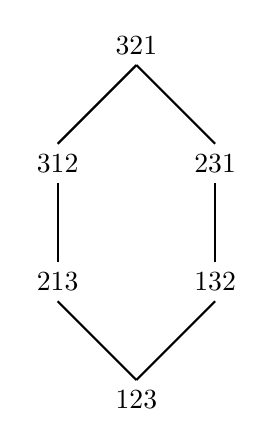
\begin{tikzpicture}[scale = .5, thick]
    \draw (3,0)--(5,2);
    \draw (3,0)--(1,2);
    \draw (5,3)--(5,5);
    \draw (1,3)--(1,5);
    \draw (1,6)--(3,8);
    \draw (5,6)--(3,8);
    \draw (3,0) node[below]{$123$};
    \draw (1,2) node[above] {$213$};
    \draw (5,2) node[above] {$132$};
    \draw (1,5) node[above] {$312$};
    \draw (5,5) node[above] {$231$};
    \draw (3,8) node[above] {$321$};
\end{tikzpicture}
~~~~~
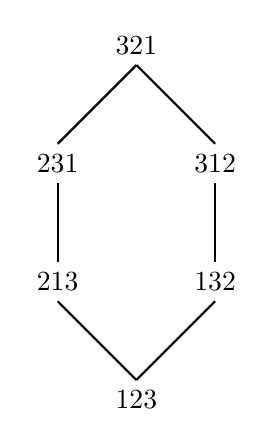
\begin{tikzpicture}[scale = .5, thick]
    \draw (3,0)--(5,2);
    \draw (3,0)--(1,2);
    \draw (5,3)--(5,5);
    \draw (1,3)--(1,5);
    \draw (1,6)--(3,8);
    \draw (5,6)--(3,8);
    \draw (3,0) node[below]{$123$};
    \draw (1,2) node[above] {$213$};
    \draw (5,2) node[above] {$132$};
    \draw (1,5) node[above] {$231$};
    \draw (5,5) node[above] {$312$};
    \draw (3,8) node[above] {$321$};
\end{tikzpicture}
\caption{The left and right weak order on $S_3$ pictured on the left and right respectively.}
\label{fig:weak-order}
\end{figure}


\section{Parke--Taylor varieties and $\monbar$} \label{sec:PTM0n}
In this section we describe some geometric properties of the Parke--Taylor variety $\mathrm{PT}_n$. In particular, we show that the open Parke--Taylor variety $\pt_n^\circ$ is isomorphic to the moduli space of $n$ marked points on the projective line, $\cm_{0,n}$. Moreover, the Parke--Taylor variety $\pt_n$ is isomorphic to the Deligne--Kundsen--Mumford compactification, $\monbar$ and thus gives a new embedding of $\monbar$ into $\pp^{(n-2)! - 1}$ which is linearly isomorphic to the well known embedding of Keel and Tevelev \cite{keel2009equations}.
We then exploit this relationship between $\pt_n$ and $\monbar$ to obtain the degree and dimension of $\pt_n$. In \cref{sec:idealPT} we will further elaborate on how this structure also allows us to better understand the generators of the vanishing ideal $\ci(\pt_n)$, and thus determine polynomial relations which hold for Parke--Taylor functions. 

\newpage

\begin{theorem} \label{thm:PTM0n}
    The open Parke--Taylor variety $\mathrm{PT}^\circ_n$ is isomorphic to the moduli space $\mathcal{M}_{0,n}$. 
\end{theorem}

\begin{proof}
    Note that the map $\varphi_n: \mathrm{Gr}(2,n)\dashrightarrow \mathrm{PT}_n$ is not birational, its fibers have positive dimension. This stems from the fact that scaling the columns of a matrix representative of $V\in\mathrm{Gr}(2,n)$ does not change the point $\varphi_n(V)$ in $\mathrm{PT}_n$. This means that $\varphi_n$ induces a dominant rational map $\mu_n: \mathrm{Gr}(2,n)/(\mathbb{C}^*)^n\dashrightarrow \mathrm{PT}_n\subset \mathbb{P}^{(n-2)!-1}$. The domain $\mathrm{Gr}(2,n)/(\mathbb{C}^*)^n$ is the moduli space $\mathcal{M}_{0,n}$. The map $\mu_n$ is in fact birational. To show this, for any quadruple of indices $(i,j,k,l)$, consider two Parke--Taylor functions that correspond to permutations that only differ by the transposition $(ij)$ so that the first one involves the product $p_{ki}p_{ij}p_{jl}$ and the second one the product $p_{kj}p_{ij}p_{il}$, with all the other variables in both functions being the same. Then the ratio of these two Parke--Taylor functions is the cross-ratio $[ij|kl]=\dfrac{p_{ik}p_{jl}}{p_{jk}p_{il}}$. In case one of the Parke--Taylor functions in this ratio corresponds to a permutation that does not fix $1$ and $2$, we express it a linear combination of the Parke--Taylor functions that have this property. These cross-ratios define a unique point of $\mathcal{M}_{0,n}$ \cite[Proposition 1.6]{lam2024moduli}, which shows that $\mu_n$ is invertible on $\mathrm{PT}^\circ_n$, i.e. is an isomorphism between $\mathcal{M}_{0,n}$ and $\mathrm{PT}^\circ_n$. Since $\mathcal{M}_{0,n}$ is a rational variety and $\mathrm{PT}^\circ_n$ is open and Zariski dense in $\mathrm{PT}_n$, the variety $\mathrm{PT}_n$ is rational and in particular irreducible. 
\end{proof}

\begin{remark}
\label{rem:restrict-to-m0n}
One consequence of the above theorem is that we may restrict the domain of the parametrization $\varphi_n$ to $\cm_{0, n}$ without changing the image. Recall that $\cm_{0, n}$ can be identified with the subset of $\gr(2, n)$ whose elements are represented by matrices of the form:
\[
\begin{pmatrix}
    1 & 1 & 1 & \cdots & 1 & 1\\
    p_1 & p_2 & p_3 & \cdots &p_{n-1} &p_n
\end{pmatrix},
\]
where one puts $p_1=0,\ p_2=1,\ p_n=\infty$ (this last equality can also be interpreted as replacing the last column with $(0\ 1)^T$) and $p_i\neq p_j$.
The Pl\"ucker embedding of a matrix of this form is then of course given by $p_{ij} = p_i - p_j$ and so $\varphi_n$ can be rewritten as
\begin{align*}
\varphi_n: \cm_{0, n} &\to \pp^{(n-2)! - 1} \\
            (p_1, \ldots p_n) &\mapsto \left(  \prod_{i=1}^n \dfrac{1}{p_{\sigma_i} - p_{\sigma_{i+1}}}  ~:~ \sigma \in \Sigma_n \right).
\end{align*}
Throughout the remainder of this paper we will abuse notation and denote by $\varphi_n$ the map which appears in \cref{def:pt} and that which is above, as the images of these maps coincide. 
\end{remark}


Since $\mathrm{PT}_n^\circ$ is isomorphic to $\cm_{0, n}$, a natural next question is to determine if the closure, $\pt_n$ is isomorphic to the corresponding closure $\monbar$. Surprisingly, this is indeed the case and thus the parametrization of the Parke--Taylor variety in \Cref{def:pt} gives a new embedding of $\monbar$. We show this by exhibiting a linear isomorphism between $\pt_n$ and the \emph{log canonical embedding} of $\monbar$ introduced by Keel and Tevelev \cite{keel2009equations}. We begin with a brief overview of the log canonical embedding of $\monbar$. For a more detailed description, we refer to \cite{keel2009equations, monin2017equations}. 


Recall that the moduli space $\monbar$ parametrizes \emph{stable $n$-pointed rational curves} which are represented as tuples $(C, p_1, \ldots, p_n)$. In \cite{keel2009equations}, the authors introduced a map $\Omega_n$, called the \emph{iterated Kapranov embedding} which embeds $\monbar$ into the product of projective spaces $\pp^1 \times \pp^2 \times \cdots \times \pp^{n-3}$. This map naturally arises from repeatedly applying the Kapranov morphism $\Psi_n: \overline{\cm_{0, n}} \to \pp^{n-3}$ which was introduced in \cite{kapranov1993veronese} and the forgetful map $\pi_n: \monbar \to \overline{\cm_{0, n-1}}$ which is given by forgetting the last point $p_n$ and stabilizing the curve $C$. The following theorem of \cite{keel2009equations} will allow us to describe $\Omega_n$ explicitly in coordinates. 


\begin{theorem}\cite[Corollary 2.7]{keel2009equations}
The map $\Omega_n: \monbar \to \pp^1 \times \pp^2 \times \cdots \times \pp^{n-3}$ is a closed embedding. 
\end{theorem}


As noted in \cite{monin2017equations}, since $\cm_{0, n}$ is Zariski dense in $\monbar$, and $\Omega_n$ is a closed embedding, it suffices to describe $\Omega_n$ on $\cm_{0, n}$. Throughout the remainder of this section we will use the following explicit description of the log canonical embedding due to \cite{monin2017equations}. 


\begin{definition}\cite{keel2009equations}
The \emph{log canonical embedding} $\Phi_n$ of $\monbar$ is the composition of the Segre embedding $\xi$ of $\pp^1 \times \pp^2 \times \cdots \times \pp^{n-3}$ with the \emph{iterated Kapranov embedding} $\Omega_n$ which is
\begin{align*}
\Omega_n: \monbar &\to \pp^1 \times \pp^2 \times \cdots \times \pp^{n-3} 
\end{align*}
where for a tuple $(C, p_1, \ldots, p_n) \in \cm_{0, n}$ the $i$-th component is given by $(\Omega_n(C, p_1, \ldots, p_n))_i = [\frac{p_1 -p_2}{p_{i+3}-p_2}:\cdots:\frac{p_1 -p_{i+2}}{p_{i+3}-p_{i+2}}]$. We denote the closure of the image of $\Phi_n$ by $\lc_n = \overline{\mathrm{image}(\Phi_n))}$. 
\end{definition}


\begin{example}
\label{ex:log-canon-5}
Consider the case $n = 5$ in which the log canonical embedding $\Phi_n$ is given by the composition $\Phi_5 = \xi  \circ  \Omega_5$ where $\xi$ is the Segre embedding of $\pp^1 \times \pp^2$ and $\Omega_5: \overline{\cm_{0, 5}} \to \pp^1 \times \pp^2$ is the iterated Kapranov embedding which is given by
\[
\Omega_5(p_1 \ldots, p_5) = \left[\frac{p_1 - p_2}{p_4 - p_2} : \frac{p_1 - p_3}{p_4 -p_3}\right], \left[\frac{p_1 - p_2}{p_5 - p_2} : \frac{p_1 - p_3}{p_5 -p_3} : \frac{p_1 - p_4}{p_5 -p_4}\right]
\]
for 5 marked points $(p_1, \ldots, p_5) \in \cm_{0, n}$. Applying the Segre embedding to the image of $\Omega_5$, yields the log canonical embedding which is then given by
\begin{align*}
t_{11} = \frac{(p_1 - p_2)^2}{(p_4 - p_2)(p_5 - p_2)},~~  t_{12} = \frac{(p_1 - p_2)(p_1 - p_3)}{(p_4 - p_2)(p_5 - p_3)},~~  t_{13} = \frac{(p_1 - p_2)(p_1 - p_4)}{(p_4 - p_2)(p_5 - p_4)},\\
t_{21} = \frac{(p_1 - p_3)(p_1 - p_2)}{(p_4 - p_3)(p_5 - p_2)},~~  t_{22} = \frac{(p_1 - p_3)^2}{(p_4 - p_3)(p_5 - p_3)},~~ t_{23} = \frac{(p_1 - p_3)(p_1 - p_4)}{(p_4 - p_3)(p_5 - p_4)}.
\end{align*}

One can verify with direct computation in a computer algebra system such as \texttt{Macaulay2} \cite{M2}, that the vanishing ideal of $\lc_5 = \mathrm{image}(\Phi_5)$ is generated by the 5 quadratics which appeared in \cite[Corollary 1.3]{monin2017equations}:
\begin{align*}
\ci(\lc_5) =  
\langle
t_{11}t_{12}-t_{12}t_{13}-t_{11}t_{22}+t_{11}t_{23}, t_{12}t_{21}-t_{21}t_{22}-t_{12}t_{23}+t_{21}t_{23}\\
-t_{11}t_{22}+t_{13}t_{22}+t_{21}t_{22}-t_{21}t_{23}, -t_{13}t_{21}+t_{11}t_{23}, t_{13}t_{22}-t_{12}t_{23}
\rangle. 
\end{align*}
Moreover, since this ideal is codimension 3 and is Gorenstein, there exists an antisymmetric matrix such that the ideal is generated by its $4 \times 4$ sub-Pfaffians \cite[Theorem 2.1]{buchsbaum1977algebra}. For $\ci(\lc_5)$, the following matrix realizes this result: 
\begin{align*}
M_\lc = \begin{pmatrix}
0& 0& t_{22}-t_{23}& -t_{11}+t_{13}& -t_{21}+t_{23} \\
0& 0&-t_{12}+t_{22}-t_{23}& t_{13}& t_{23} \\
-t_{22}+t_{23}& t_{12}-t_{22}+t_{23}& 0& -t_{22}+t_{23}& -t_{22} \\
t_{11}-t_{13}&-t_{13}& t_{22}-t_{23}& 0& t_{23} \\
t_{21}-t_{23}& -t_{23}& t_{22}&-t_{23}& 0
\end{pmatrix}.
\end{align*}
\end{example}


The second ingredient which we require to state our main theorem of this section is the following definition which we use in the construction of our linear map between $\lc_n$ and~$\pt_n$. 


\begin{definition}
\label{defn:shuffle-sum}
Let $\inv(\sigma)$ denote the set of value-wise inversions set of $\sigma$, which is given by $\inv(\sigma) = \{(\sigma_i, \sigma_j) ~:~  i < j \text{ and } \sigma_i > \sigma_j \}$. Then for any $i \in [n-3]$ and $\sigma \in \Sigma_{n-1}$, let $\shuffle_i z_\sigma \in \cc[z_\tau ~:~ \tau \in \Sigma_n
]$ be the linear polynomial
\[
\displaystyle \shuffle_{i} z_\sigma = \sum_{\substack{\tau \in \Sigma_n \\ \tau \setminus \{n \} = \sigma \\ (i, n) \notin \inv(\tau)}} z_\tau. 
\]
\end{definition}



\begin{theorem}
\label{thm:log-canon-Parke--Taylor}
The Parke--Taylor variety $\pt_n$ is linearly isomorphic to the log canonical embedding $\lc_n$ and thus is a closed embedding of $\monbar$ into $\pp^{(n-2)! - 1}$. For $n \geq 6$, the linear isomorphism is given by the equations
\[
t_{i_1 \ldots i_{n-3}} = \sum_{\sigma \in B_{i_1 \ldots i_{n-4}}} \shuffle_{i_{n-3}+1} z_\sigma
\]
where $B_{i_1 \ldots i_{n-4}}$ is defined by $t_{i_1 \ldots i_{n-4}} = \sum_{\sigma \in B_{i_1 \ldots i_{n-4}}} z_\sigma$.
\end{theorem}

We delay the proof of this theorem and first give an example for $n = 5$ which serves as the base case for the iterative construction described in the theorem statement. 


\begin{example}
\label{ex:LC-to-PT-5}
Let $\pt_5$ and $\lc_5$ be the closed Parke--Taylor variety and the log canoncial embedding of $\overline{\mathcal{M}}_{0.n}$ respectively. Then the linear map $L_5$ from $\lc_5$ to $\pt_5$ is given by:
\begin{align*}
L_5(t_{11}) &= z_{12345} + z_{12354} + z_{12435} + z_{12453} + z_{12534} + z_{12543} = \sum_{\substack{\sigma \\ \inv(\sigma) \subseteq \{(2,1), (3,1), (3,2)\}}} z_\sigma,\\
L_5(t_{12}) &= z_{12345} + z_{12354} + z_{12435}  = \sum_{\substack{\sigma \\ \inv(\sigma) \subseteq \{(2,1), (3,2)\}}} z_\sigma,\\
L_5(t_{13}) &= z_{12345} + z_{12435} + z_{12453} = \sum_{\substack{\sigma \\ \inv(\sigma) \subseteq \{(2,1), (3,1) \}}} z_\sigma, \\ 
L_5(t_{21}) &= z_{12345} + z_{12354} + z_{12534} = \sum_{\substack{\sigma \\ \inv(\sigma) \subseteq \{(3,1), (3,2)\}}} z_\sigma,\\
L_5(t_{22}) &= z_{12345} + z_{12354} = \sum_{\substack{\sigma \\ \inv(\sigma) \subseteq \{(3,2)\}}} z_\sigma,\\
L_5(t_{23}) &= z_{12345} = \sum_{\substack{\sigma \\ \inv(\sigma) \subseteq \emptyset}} z_\sigma.\\
\end{align*}
Furthermore, this linear map sends the vanishing ideal $\ci(\lc_5)$ of the log canonical embedding to $\ci(\pt_5)$. Since $L_5$ is a linear map, the resulting ideal is also generated by 5 quadratics:
\begin{align*}
\ci(\pt_5) = 
\langle 
z_{12354}z_{12435}+z_{12345}z_{12453}+z_{12354}z_{12453}, z_{12345}z_{12534}+z_{12345}z_{12543}+z_{12354}z_{12543},\\
z_{12354}z_{12435}+z_{12345}z_{12534}+z_{12435}z_{12534}, z_{12345}z_{12453}+z_{12345}z_{12543}+z_{12435}z_{12543},\\
z_{12354}z_{12435}+z_{12345}z_{12534}+z_{12435}z_{12534} 
\rangle.
\end{align*}
Note that the 5 quadratics above are not exactly the images of the 5 generators of $\ci(\lc_5)$ which appear in \cref{ex:log-canon-5} but they generate the same ideal. We will provide a detailed explanation of the quadratics which appear above in \cref{sec:idealPT} but here we note
that by the same theorem of \cite{buchsbaum1977algebra}, $\ci(\pt_5)$ can also be generated by the submaximal Pfaffians of a $5 \times 5$ antisymmetric matrix. In this case the following matrix suffices:
\begin{align*}
M_\pt = \begin{pmatrix}
0& -z_{12543}& -z_{12345}& -z_{12354}-z_{12534}& z_{12345} \\
z_{12543}& 0& -z_{12435}+z_{12543}& -z_{12543}& z_{12435}+z_{12453} \\
z_{12345}& z_{12435}-z_{12543}& 0& -z_{12534}& -z_{12435} \\ 
z_{12354}+z_{12534}& z_{12543}& z_{12534}& 0& 0 \\
-z_{12345}& -z_{12435}-z_{12453}&z_{12435}& 0& 0
\end{pmatrix}. 
\end{align*}
\end{example}


At first glance, one might hope that the linear map $L_5$ corresponds to a sum over permutations in a \emph{principal} lower order ideal in the \emph{right weak order} on the symmetric group $\Sigma_n \cong S_{n-2}$ \cite{bjornerbrenticoxeter}, but this is unfortunately not the case. However, each coordinate $t_{i_1 \ldots i_n}$ does correspond to a sum over permutations in a lower order ideal in the right weak order. We will expand upon this later in this section but we first develop a few results which will be core ingredients in the proof of \cref{thm:log-canon-Parke--Taylor}. 


\begin{lemma}
\label{lemma:plucker-sum-shuffle}
Let $p_{ij}$ denote the Pl\"ucker coordinates on $\gr(2, n)$. Then for any $i$ such that $3 \leq i \leq n-1$ and $\sigma \in \Sigma_{n-1}$, it holds that
\[
\sum_{\substack{i \leq j \leq n-1}} \frac{p_{\sigma_j \sigma_{j + 1}}}{p_{\sigma_j n}p_{\sigma_{j +1} n}} = -\frac{p_{1 \sigma_i}}{p_{\sigma_i n} p_{1n}}.
\]
\end{lemma}
\begin{proof}
The statement follows from iteratively finding common denominators and applying the Pl\"ucker relations to the left hand side. Observe that the sum of the last two terms in the above sum yields
\[
-\frac{p_{1 \sigma_{n-1}}}{p_{1n} p_{\sigma_{n-1} n}} +  \frac{p_{\sigma_{n-2} \sigma_{n-1}}}{p_{\sigma_{n-2} n } p_{\sigma_{n-1} n}} = \frac{-p_{1 \sigma_{n-1}} p_{\sigma_{n- 2} n} + p_{1 n} p_{\sigma_{n- 2} \sigma_{n - 1}}}{p_{1n} p_{\sigma_{n-2} n } p_{\sigma_{n-1} n}} = \frac{-p_{1 \sigma_{n-2}} p_{\sigma_{n-1} n}}{p_{1n} p_{\sigma_{n-2} n } p_{\sigma_{n-1} n}} =  \frac{-p_{1 \sigma_{n-2}}}{p_{1n} p_{\sigma_{n-2} n }}.
\]
Repeatedly applying this technique to the output of the previous step together with the last remaining term of the original sum then yields the desired result. 
\end{proof}


\begin{corollary}
\label{cor:pt-recursive-shuffle}
Let $\varphi_n$ be the parametrization of $\pt_n$ as defined in \cref{def:pt}. Then for any $3 \leq i\leq n-1$ and $\sigma \in \Sigma_{n-1}$, it holds that
\[
\varphi_{n-1}^\ast(z_\sigma) \frac{-p_{1 \sigma_i }}{p_{\sigma_i n} p_{1n}} = \varphi_n^\ast(\shuffle_{\sigma_i} z_\sigma),
\]
where $\shuffle_{\sigma_i} z_\sigma$ is the sum defined in \cref{defn:shuffle-sum}. 
\end{corollary}
\begin{proof}
First, observe that
\[
\varphi_{n-1}^\ast(z_\sigma) \frac{p_{\sigma_i \sigma_{i + 1}}}{p_{\sigma_i n}p_{\sigma_{i +1} n}} = \varphi_n^\ast(z_\tau),
\]
where $\tau$ is the permutation obtained from $\sigma$ by inserting the new letter $n$ in between $\sigma_{i}$ and $\sigma_{i+1}$. The set of permutations $\tau$ arising this way is exactly the same as the set of $\tau \in \Sigma_n$ such that $\tau \setminus \{n\} = \sigma$ and $(\sigma_i, n) \notin \inv(\tau)$. Multiplying both sides of the equality in \cref{lemma:plucker-sum-shuffle} by $\varphi_{n-1}^\ast(z_\sigma)$ then yields
\[
\varphi_{n-1}^\ast(z_\sigma)\frac{-p_{1 \sigma_i}}{p_{\sigma_i n} p_{1n}} = \varphi_{n-1}^\ast(z_\sigma)
\sum_{\substack{i \leq j \leq n-1}} \frac{p_{\sigma_j \sigma_{j + 1}}}{p_{\sigma_j n}p_{\sigma_{j +1} n}} = \varphi_n^\ast(\shuffle_{\sigma_i} z_\sigma).
\]

\end{proof}


\begin{remark}
\label{rem:alternate-pt-shuffle}
Note that the above corollary also holds if one uses the restriction of $\varphi_n$ to $\cm_{0, n}$ as discussed in \cref{rem:restrict-to-m0n} instead of the original definition in \cref{def:pt}. In that case, the equality in the previous corollary becomes
\[
\varphi_{n-1}^\ast(z_\sigma) \frac{p_1 - p_{\sigma_i}}{(p_{n} - p_{\sigma_i}) (p_{1} - p_n)} = \varphi_n^\ast(\shuffle_{\sigma_i} z_\sigma).
\]
\end{remark}

We are now ready to complete the proof of \cref{thm:log-canon-Parke--Taylor}.

\begin{proof}[Proof of \cref{thm:log-canon-Parke--Taylor}]
Let $\varphi_n$ and $\Phi_n$ be the parametrizations of $\pt_n$ and $\lc_n$ respectively. We will construct a linear map $L_n: \cc[t_{i_1 \ldots i_{n-3}}] \to \cc[z_\sigma ~:~ \sigma \in \Sigma_n ]$ such that $\varphi_n^\ast(L_n(t_{i_1 \ldots i_{n-3}})) = \Phi_n^\ast(t_{i_1 \ldots i_{n-3}})$
and thus $L_n$ maps $\pt_n^\circ$ to $\lc_n^\circ$. Since both the open Parke--Taylor variety and log canonical embedding are of course Zariski dense in their corresponding closures, this implies that $L_n$ maps $\pt_n$ to $\lc_n$ as required. 

Suppose by way of induction that we already have a linear isomorphism $L_{n-1}$ between $\lc_{n-1}$ and $\pt_{n-1}$ of the required form and define $L_n$ by
\[
L_n(t_{i_1 \ldots i_{n-3}}) = \sum_{\sigma \in B_{i_1 \ldots i_{n-4}}} \shuffle_{i_{n-3} + 1} z_\sigma 
\] 
where $B_{i_1 \ldots i_{n-1}}$ is defined by $L_{n-1}(t_{i_1 \ldots i_{n-4}}) = \sum_{\sigma \in B_{i_1 \ldots i_{n-4}}} z_\sigma$. Since $\Phi_n$, is the composition of the iterated Kapranov embedding and the Segre embedding, we have that
\begin{equation}
\label{eqn:recursive-log-canon}
\Phi_n^\ast(t_{i_1 \ldots i_{n-3}})= \Phi_{n-1}^\ast(t_{i_1 \ldots i_{n-4}}) \frac{p_1 - p_{i_n + 1}}{p_n - p_{i_n + 1}} = 
\Phi_{n-1}^\ast(t_{i_1 \ldots i_{n-4}}) \frac{p_1 - p_{i_n + 1}}{(p_n - p_{i_n + 1})(p_1 - p_n)}
\end{equation}
Where the last equality simply corresponds to the fact that the domain of the Segre embedding is the product of projective spaces $\pp^1 \times \pp^2 \times \cdots \times \pp^{n-3}$ and thus we may scale the last component by $\frac{1}{p_1 - p_n}$ without changing the corresponding point in projective space. By our induction hypothesis, we have that
\begin{equation*}
\Phi_{n-1}^\ast(t_{i_1 \ldots i_{n-4}}) = \varphi_{n-1}^\ast(L_{n-1}(t_{i_1 \ldots i_{n-4}})) = \varphi_{n-1}^\ast \left(\sum_{\sigma \in B_{i_1 \ldots i_{n-4}}} z_\sigma \right)
\end{equation*}
and combining this equation with \Cref{eqn:recursive-log-canon} yields
\[
\Phi_n^\ast(t_{i_1 \ldots i_{n-3}}) = \varphi_{n-1}^\ast \left(\sum_{\sigma \in B_{i_1 \ldots i_{n-4}}} z_\sigma \right) \frac{p_1 - p_{i_n + 1}}{(p_n - p_{i_n + 1})(p_1 - p_n)} = \varphi_n^\ast \left( \sum_{\sigma \in B_{i_1 \ldots i_{n-4}}} \shuffle_{i_{n-3}+ 1} z_\sigma \right),
\]
where the last equality follows immediately by applying \cref{cor:pt-recursive-shuffle}, or more specifically the alternative version of it stated in \cref{rem:alternate-pt-shuffle}. This completes the proof since the right hand side of the above equation is $\varphi_n^\ast(L_n(t_{i_1 \ldots i_{n-3}}))$ by definition.  
\end{proof}

The following example showcases the iterative construction of the map $L_n$. 

\begin{example}
\label{ex:iterative-LC-to-PT}
Let $n = 6$ and recall from \Cref{ex:LC-to-PT-5} that $L_5(t_{21}) = z_{12345} + z_{12354} + z_{12534}$. Then $i_{n-3} = 2$ and so $L_6(t_{212})$ is given by
\begin{align*}
L_6(t_{212}) &= \sum_{\sigma \in B_{21}} \shuffle_{3} z_\sigma =  \underline{\textcolor{red}{\shuffle_3 z_{12345}}} + \underline{\underline{\textcolor{blue}{\shuffle_3 z_{12354}}}}+ \textcolor{ForestGreen}{\shuffle_3 z_{12534}}\\
&= \underline{\textcolor{red}{z_{123456} + z_{123465} + z_{123645}}} + \underline{\underline{\textcolor{blue}{z_{123546} + z_{123564} + z_{123654}}}}  + \textcolor{ForestGreen}{z_{125346} + z_{125364}}, 
\end{align*}
where the colored (or underlined) terms in the second line are the corresponding expansion of those in the first. As explained in the proof of \cref{cor:pt-recursive-shuffle}, note that $\shuffle_{3} z_\sigma$ can also be thought of as a sum over all permutations $\tau$ such that $\tau$ is obtained from $\sigma$ by inserting $6$ in to $\sigma$ at any position after $3$. 
\end{example}


The following result clarifies the relationship between the support sets $B_{i_1 \ldots i_{n-3}}$, which encode the linear map $L_n$ between $\pt_n$  and $\lc_n$, and the the \emph{right weak order} on permutations. 


\begin{proposition}
The set $B_{i_1, \cdots i_{n-3}}$ is a lower order ideal in the right weak order. Moreover, $B_{i_1, \ldots i_{n-3}} = \{\sigma \in \Sigma_n ~:~ \inv(\sigma) \subseteq S \cup T\}$ where
$S$ is defined recursively by $B_{i_1, \ldots i_{n-4}} = \{\sigma' \in \Sigma_{n-1} ~:~ \inv(\sigma') \subseteq S\}$ and $T = \{(i, n) ~:~ \text{there exists } \tau \in B_{i_1 \ldots i_{n-4}}, ~~\tau^{-1}(i) > \tau^{-1}(i_{n-3} + 1) \}$.
\end{proposition}
\begin{proof}
We first show that $B_{i_1, \cdots i_{n-3}}$ is indeed a lower order ideal in the weak order by induction on $n$. Observe that for $n = 5$ this is indeed the case and assume the result holds for $B_{i_1 \ldots i_{n-4}}$. 
Now suppose that $\sigma \in B_{i_1 \ldots i_{n-3}}$ and $\tau \leq \sigma$ in the right weak order on $\Sigma_{n}$. So we must show that $\tau \in B_{i_1 \ldots i_{n-3}}$. Let $\tau' = \tau \setminus \{n\} \in \Sigma_{n-1}$ be the permutation obtained from $\tau$ by deleting $n$ and define $\sigma'$ analogously. Then by definition of the weak order, it must be that $\tau' \leq \sigma'$ and since $\sigma \in B_{i_1 \ldots i_{n-3}}$, it must be that $\sigma' \in B_{i_1 \ldots i_{n-4}}$. 
By the inductive hypothesis, $\tau' \in B_{i_1 \ldots i_{n-4}}$ and thus we see that $\tau \in B_{i_1 \ldots i_{n-3}}$ which shows that $B_{i_1 \ldots i_{n-3}}$ is indeed a lower order ideal. 

To prove the second statement, we also proceed by induction with $n = 5$ serving as the base case. Let $S$ and $T$ be defined as above and let $C_{i_1 \ldots i_{n-3}} = \{\sigma \in \Sigma_n ~:~ \inv(\sigma) \subseteq S \cup T\}$. Clearly it holds that $B_{i_1 \ldots i_{n-3}} \subseteq C_{i_1 \ldots i_{n-3}}$ so it remains to show the reverse inclusion. So suppose that $\sigma \in C_{i_1 \ldots i_{n-3}}$ and observe that $\sigma' = \sigma \setminus \{n\} \in B_{i_1 \ldots i_{n-4}}$ since $\inv(\sigma') = \inv(\sigma) \setminus T \subseteq S$. But this once again immediately implies that $\sigma \in B_{i_1 \ldots i_{n-3}}$ since $(i_{n-3}+1, n) \notin \inv(\sigma)$.  
\end{proof}


The fact that $B_{i_1 \ldots i_{n-3}}$ can be described as a set of permutations whose inversions sets are all contained in a given set of inversions is actually quite special and does not hold for every lower order ideal of the weak order. For example if one considers the lower order ideal in the weak order on $S_3$ generated by the permutations $231$ and $312$ as pictured in \Cref{fig:weak-order}, then $\inv(321) = \inv(231) \cup \inv(312) = \{(1,2), (1,3), (2,3)\}$ however $321 \notin \langle 231, 312 \rangle$.



We now use the linear isomorphism between $\mathrm{PT}_n$ and $\mathrm{LC}_n$ to derive some properties of $\pt_n$ and its defining ideal. We note that the multidegree of the embedding $\Omega_n$ of $\monbar$ into $\mathbb{P}^1\times\ldots\times \mathbb{P}^{n-3}$ was computed in \cite{cavalieri2021projective}. The multidegree of a smooth subvariety of a product of projective spaces can be easily transformed into the degree of its image under the Segre embedding, leading to the following result. We write $\binom{n}{i_1\ldots i_{r}}$ for the usual multinomial coefficient and $\abinom{n}{i_1\ldots i_{r}}$ for the asymmetric multinomial coefficient (see \cite[Definition 4.11]{cavalieri2021projective}).

\begin{corollary} \label{cor:degree}
The degree of $\lc_n$, and thus $\pt_n$, is
$$\sum\limits_{i_1+\ldots+i_{n-3}=n-3} \binom{n-3}{i_1\ldots i_{n-3}}\abinom{n-3}{i_1\ldots i_{n-3}}.$$
\end{corollary}

\begin{proof}
    The coefficient $d_{i_1,\ldots,i_{n-3}}$ of the multidegree polynomial of $\Omega_n(\monbar)$ is the asymmetric multinomial coefficient $\abinom{n-3}{i_1\ldots i_{n-3}}$ by \cite[Theorem 1.1]{cavalieri2021projective}. Let $\xi$ denote the Segre embedding $\mathbb{P}^1\times\ldots\times \mathbb{P}^{n-3}\hookrightarrow \mathbb{P}^{(n-2)!-1}$.  Write $h_i=c_1(\mathcal{O}_{\mathbb{P}^i}(1))$, where 
    $c_1$ is the first Chern class. Then we have $c_1(\xi^*\mathcal{O}_{\mathbb{P}^{(n-2)!-1}}(1))=h_1+\ldots+h_{n-3}$ (see e.g. \cite[Equation (3.5)]{kozhasov2023minimal}). The degree of $\mathrm{LC}_n$ is given by 
    \begin{multline*}
        \deg \mathrm{LC}_n = \int\limits_{\mathbb{P}^{(n-2)!-1}} c_1(\xi^*\mathcal{O}_{\mathbb{P}^{(n-2)!-1}}(1))^{n-3}\cap[\mathrm{LC}_n] = \int\limits_{\mathbb{P}^{(n-2)!-1}}(h_1+\ldots+h_{n-3})^{n-3}\cap [\mathrm{LC}_n] =\\ =\sum\limits_{i_1+\ldots+i_{n-3}=n-3} \binom{n-3}{i_1\ldots i_{n-3}}d_{i_1\ldots i_{n-3}}=\sum\limits_{i_1+\ldots+i_{n-3}=n-3} \binom{n-3}{i_1\ldots i_{n-3}}\abinom{n-3}{i_1\ldots i_{n-3}}.\end{multline*}
Since $\mathrm{PT}_n$ is linearly isomorphic to $\mathrm{LC}_n$ by \cref{thm:log-canon-Parke--Taylor}, its degree is the same. 
\end{proof}

\begin{example}
For $n=5$ the only nonzero asymmetric multinomial coefficients are $\abinom{2}{20} = 1$ and $\abinom{2}{1 1}=2$. Plugging these into the formula from \cref{cor:degree} yields $\deg \pt_5 = 5$. For $n=6$ we have $\abinom{3}{111}=6$, $\abinom{3}{120}=3$, $\abinom{3}{3 0 0 } = 1$, $\abinom{3}{2 0 1}=2$ and $\abinom{3}{210}=3$. This then yields $\deg\pt_6 = 6\cdot 6+ 3\cdot 3+ 1\cdot 1+ 2\cdot3 + 3\cdot 3 = 61$. We also verified these numbers by a computation in \texttt{Macaulay2}. 
\end{example}


\begin{proposition}\cite[Theorem 8.6]{keel2009equations}
The ideal $\ci(\lc_n)$ is quadratically generated. 
\end{proposition}


\begin{corollary}
The ideal $\ci(\pt_n)$ is quadratically generated. 
\end{corollary}



This corollary follows immediately from the fact that $\ci(\lc_n)$ is quadratically generated and the fact that $\pt_n$ is linearly isomorphic to $\lc_n$. 
While both $\lc_n$ and $\pt_n$ are quadratically generated embeddings of $\monbar$, we will see in the following sections that the ways in which the quadratic generators of their respective ideals arise are quite different from an algebraic perspective. In particular we will show that our parametrization $\varphi_n$ of $\pt_n$ can also be seen as the composition of a monomial map $\tilde{\varphi}_n$ which we study in \cref{sec:toric} and the Pl\"ucker embedding whereas the log canonical embedding $\Phi_n$ is the composition of the Segre embedding and the iterated Kapranov embedding $\Omega_n$. From this perspective one can see that
\[
\ci(\pt_n) = (\tilde{\varphi_n}^\ast)^{-1}(\ci(\gr(2,n))), ~~ \ci(\lc_n) = (\psi^\ast)^{-1}(\ker(\Omega_n^\ast)).
\]
In the case of $\pt_n$, the monomial map $\tilde{\varphi}_n$, and its associated toric ideal are quite complicated as we will see in the next section, but the ideal $\ci(\gr(2,n))$, which we must compute the preimage of, is quite simple and it is well known that it is generated by the Pl\"ucker relations. On the other hand, for $\lc_n$, the Segre embedding is an extremely simple monomial map and its corresponding toric ideal is generated by quadratic binomials, however $\ker(\Omega_n^\ast)$ is more complicated and is generated by the cubics known as the \emph{Monin--Rana} equations \cite{gillespie2022proof, monin2017equations}. 


\section{Binomial Parke--Taylor identities} \label{sec:toric}
In this section we describe a variety $T_n$ that contains $\mathrm{PT}_n$ and is cut out by binomial equations. Note that due to the containment, every equation of $T_n$ vanishes on $\mathrm{PT}_n$, that is we have the corresponding reverse containment of ideals $\ci(T_n) \subseteq \ci(\pt_n)$. Therefore, this is the first step to describing the ideal of $\mathrm{PT}_n$.

We first describe $T_n$ geometrically. The Grassmannian $\mathrm{Gr}(2,n)$ is embedded into the projective space $\mathbb{P}^{\binom{n}{2}-1}$ with coordinates $p_{ij}$. We can therefore extend the map $\varphi_n: \mathrm{Gr}(2,n)\dashrightarrow \mathbb{P}^{(n-2)!-1}$ from Definition \ref{def:pt} to a rational map $\tilde{\varphi}_n:\mathbb{P}^{\binom{n}{2}-1}\dashrightarrow \mathbb{P}^{(n-2)!-1}$ on the whole projective space given by the same formula. We define $T_n$ to be the Zariski closure of the image of $\tilde{\varphi}_n$. Observe that this implies that $\mathrm{PT}_n$ is a subvariety of $T_n$ since $\varphi_n$ is simply the restriction of $\tilde{\varphi}_n$ to the Grassmanian.  

The map $\tilde{\varphi}_n$ yields a very special parametrization of $T_n$: it is given by monomials. Varieties parametrized by monomials are called \emph{toric}. This very special class of varieties is extremely well-studied in the literature, see \cite{cox2011toric} for a comprehensive reference. As explained in \cite[Section 3.3]{Lam2022PosGeom}, toric varieties also naturally give a class of positive geometries. We begin our investigation of this toric variety with the following result concerning its dimension. In what follows, we use the term \emph{affine cone}, which is the affine variety in $\mathbb{C}^{(n-2)!}$ cut out by the same equations as the projective variety $T_n\subseteq \mathbb{P}^{(n-2)!-1}$. The generators of the ideal of a projective variety and of its affine cone are the same. 


\begin{proposition} \label{prop:toricdim}
    The affine cone over the toric variety $T_n$ is an irreducible variety of affine dimension $\binom{n-1}{2}-1$.
\end{proposition} 
\begin{proof}
Note that the map $\tilde{\varphi}_n$ also parametrizes the affine cone over $T_n$ when considered as a map from $\cc^{\binom{n}{2}} \to \cc^{(n-2)!}$. 
Thus our strategy is to indicate an affine space of dimension $\binom{n-1}{2}-1$ in $\mathbb{P}^{\binom{n}{2}-1}$, which yields a subspace of $\cc^{\binom{n}{2}}$, on which $\tilde{\varphi}_n$ is dominant and invertible. 
    
    Consider the affine space $W\subset\mathbb{P}^{\binom{n}{2}-1}$ defined by the $n$ independent equations $p_{1,2}=1$ and $p_{i,n}=1$ for $i\in[n-1]$. The coordinates on $W$ are then $p_{ij}$ with $1\leq i<j<n$ and $(i,j)\neq(1,2)$ . As shown in the proof of Theorem \ref{thm:PTM0n}, any cross-ratio $[ij|kl] = \dfrac{p_{ik}p_{jl}}{p_{jk}p_{il}}$ is a ratio of two Parke--Taylor functions. On $W$ we have $[1n|2j]=\dfrac{1}{p_{1j}}$ for $2<j<n$ and $\dfrac{[1n|2j]}{[1i|jn]}=p_{ij}$ for $1<i<j<n$. Thus, every $p_{ij}$ is a ratio of polynomial combinations of Parke--Taylor functions, and $\tilde{\varphi}_n|_W$ is generically invertible. Since $\dim W=\binom{n-1}{2}-1$, the proposition follows.
\end{proof}

One particularly nice feature of toric varieties is that much of their structure can be understood through the lens of polyhedral combinatorics and linear algebra, without diving into the abstract machinery of algebraic geometry. More specifically, the monomial map which parameterizes the toric variety can be encoded by an integer matrix. 


\begin{definition}
Let $A \in \zz^{d \times r}$ be an integer matrix and let $a_j$ denote the $j$-th column of $A$. Then the \emph{affine toric variety} $V_A$ associated to $A$ the matrix is the Zariski closure of the image of the map
\begin{align*}
\varphi_A : \cc^d &\to \cc^r, \\
             t  &\mapsto (t^{a_1}, t^{a_2}, \ldots, t^{a_r}),
\end{align*}
where $t^{a_j} = \prod_{i = 1}^d t_i^{a_{ij}}$. That is, $V_A = \overline{\mathrm{image}(\varphi_A)}$. The \emph{toric ideal} associated to $A$ is denoted $I_A = \mathcal{I}(V_A)$. 
\end{definition}

Observe that every toric variety can be written in the above form by taking the $j$-th column of $A$ to be the exponent vector of the $j$-th monomial. In the case of the toric Parke--Taylor  variety $T_n$, the corresponding matrix is $A_n \in \zz^{\binom{n}{2} \times (n-2)!}$ whose rows are naturally indexed by subsets $\{i, j\}\subset[n]$ and columns are indexed by permutations $\sigma \in \Sigma_n$ with entries given by
\[
(A_n)_{\{i, j\}, \sigma} =
\begin{cases}
1, \mbox{ if } i \mbox{ and } j \mbox{ are adjacent in } \sigma \\
0, \mbox{ otherwise}
\end{cases}
\]
It is then immediate from the definition that $\tilde{\varphi}_n = \varphi_{A_n}$. This perspective on toric varieties is exceedingly useful for many reasons. First, it can be shown that the ideal of defining equations of $T_n$, i.e. the \emph{toric ideal} $\ci(T_n)$, is a prime ideal generated by binomials \cite[Chapter 4]{sturmfels1996groebner} and that the dimension of $T_n$ is equal to the rank of $A_n$. Moreover, the elements in the integer kernel of the matrix $A_n$ immediately yield many binomial relations in the ideal. 

\begin{proposition}\cite[Chapter 4]{sturmfels1996groebner}
Let $A \in \zz^{d \times r}$ be an integer matrix and $I_A$ be the associated toric ideal. Then
\[
I_A = \langle z^u - z^v ~:~ u, v \in \zz_{\geq 0}^r \mbox{ and } Au = Av \rangle.
\]
\end{proposition}

In other words, the toric ideal gives an encoding of the integer kernel, $\ker_\zz(A)$. Every binomial $x^{u} - x^v \in I_A$ gives rise to a vector $u - v \in \ker_\zz(A)$ and any vector $u \in \ker_\zz(A)$ can be written as $u = u^+ - u^-$ for vectors $u^+, u^- \in \zz_{\geq 0}^r$ which naturally corresponds to a binomial $x^{u^+} - x^{u^-} \in I_A$. In our Parke--Taylor setting, the variables parametrizing $T_n$ are labeled by adjacencies of permutations on $[n]$, which immediately yields following result.

\begin{proposition}
\label{prop:toric-gens-via-adjs}
A binomial equation of the form 
$$\prod\limits_{\sigma\in A} z_\sigma - \prod\limits_{\tau\in B} z_\tau = 0$$
holds on $T_n$ if and only if the set of adjacencies of all permutations in $A$ (counted with multiplicity) is the same as the set of adjacencies of all permutations in $B$. Moreover, the set of all such binomials above generates $\ci(T_n)$. 
\end{proposition}

This simple combinatorial rule immediately allows to construct many nonlinear Parke--Taylor relations as we will shortly demonstrate. First, we introduce two important notations which will be useful throughout the rest of this paper. For a permutation $\sigma = \sigma_1 \sigma_2 \cdots \sigma_n$ in one-line notation, we denote the adjacency of $\sigma_i$ and $\sigma_{i+1}$ by $\sigma_{i}\sigma_{i+1}$.

Next, in the following results we will often use the \emph{tableau notation} of a binomial in which we write
\[
\prod\limits_{\sigma\in A} z_\sigma - \prod\limits_{\tau\in B} z_\tau = 
\begin{bmatrix}
1 & 2 & \cdots & \sigma_i^{(1)} &  \cdots & \sigma_n^{(1)} \\
1 & 2 & \cdots & \vdots         & \cdots & \vdots  \\
1 & 2 & \cdots & \sigma_i^{(m)} & \cdots & \sigma_n^{(m)} \\
\end{bmatrix} - 
\begin{bmatrix}
1 & 2 & \cdots & \tau_i^{(1)} & \cdots & \tau_n^{(1)} \\
1 & 2 & \cdots & \vdots       & \cdots & \vdots  \\
1 & 2 & \cdots & \tau_i^{(m)} & \cdots & \tau_n^{(m)} \\
\end{bmatrix}. 
\]
where $A = \{\sigma^{(1)}, \ldots, \sigma^{(m)}\}$ and $\sigma^{(\ell)} = 12\sigma_{3}^{(\ell)}\sigma_{4}^{(\ell)}\cdots\sigma_{n}^{(\ell)}$ and $B$ is defined analogously. 


\begin{example}
\label{example:toric-5}
Consider the toric Parke--Taylor variety $T_5$ whose associated integer matrix is
\[
A_5 = 
\begin{blockarray}{ccccccc}
& 12345 & 12354 & 12435 & 12453 & 12534 & 12543 \\
\begin{block}{c(cccccc)}
p_{12} &1&1&1&1&1&1\\
p_{13} &0&0&0&1&0&1\\
p_{14} &0&1&0&0&1&0\\
p_{15} &1&0&1&0&0&0\\
p_{23} &1&1&0&0&0&0\\
p_{24} &0&0&1&1&0&0\\
p_{25} &0&0&0&0&1&1\\
p_{34} &1&0&1&0&1&1\\
p_{35} &0&1&1&1&1&0\\
p_{45} &1&1&0&1&0&1\\
\end{block}
\end{blockarray}.
\]
As explained above, the column corresponding to $\sigma$ is the exponent vector of the monomial which parametrizes the coordinate $z_\sigma$. For example, the identity permutation $\sigma = 12345$ corresponds to the first column $a_1$ of $A_5$. Thus, we get
\[
z_{12345} = p^{a_1} = p_{12}^1 p_{13}^0 p_{14}^0 p_{15}^1 p_{23}^1 p_{24}^0 p_{25}^0 p_{34}^1 p_{35}^0 p_{45}^1 = p_{12}p_{23}p_{34}p_{45}p_{15}. 
\]

Since $\rank(A_5) = \dim(T_n) = 5$, we know that $\ci(T_n)$ must be a principal ideal, meaning an ideal which is generated by a single polynomial. Thus, the kernel of $A_5$ is one-dimensional and is spanned by the vector 
\[
u = (1, -1, -1, 1, 1, -1) = (1, 0, 0, 1, 1, 0) - (0, 1, 1, 0, 0, 1) = u^+ - u^-.
\]
This vector corresponds to the binomial
\[
z^{u^+} - z^{u_{-}} = z_{12345}z_{12453}z_{12534} - z_{12354}z_{12435}z_{12543} = 
\begin{bmatrix}
1 & 2 & 3 & 4 & 5 \\
1 & 2 & 4 & 5 & 3 \\
1 & 2 & 5 & 3 & 4 \\
\end{bmatrix} - 
\begin{bmatrix}
1 & 2 & 3 & 5 & 4 \\
1 & 2 & 4 & 3 & 5 \\
1 & 2 & 5 & 4 & 3 \\
\end{bmatrix}.
\]
Observe that the multiset of adjacencies $\{12^3, 13, 14, 15, 23, 24, 25, 34^2, 35^2, 45^2\}$ is indeed the same in each term of this binomial. 
\end{example}

In Proposition \ref{prop:toric-gens-via-adjs} and Example \ref{example:toric-5} we saw that a binomial is in the toric ideal $I_n$ if and only if the corresponding difference of exponent vectors belongs to the kernel of the matrix $A_n$. In the previous example, the ideal was \emph{principal}, and thus a basis for the integer kernel of $A_n$ actually yielded our lone generator of the ideal. However, this is not generally the case and we might need many more binomials to generate $\ci(T_n)$. This is illustrated by the following example. 

\begin{example}
\label{example:toric-6}
The toric ideal $\ci(T_6) \subseteq \kk[z_\sigma ~:~ \sigma \in \Sigma_6]$ is minimally generated by 24 quadratics, 164 cubics, and 6 quartics which yields a total of 194 minimal generators. However, $A_6 \in \zz^{15 \times 24}$ is rank 9 and thus the kernel is minimally generated by only 15 integer vectors. The integer kernel can be generated by vectors corresponding to 15 vectors which encode only quadratic and cubic relations. In particular the following polynomials correspond to one choice of basis for $\ker_\zz(A_n)$:
\begin{align*}
z_{123465}z_{124536}-z_{123456}z_{124635}, z_{123546}z_{124365}-z_{123456}z_{124635},\\
z_{123456}z_{125364}-z_{123546}z_{125634}, z_{123456}z_{126453}-z_{123546}z_{126543},\\ 
z_{123456}z_{125364}-z_{123564}z_{125436}, z_{123564}z_{126345}-z_{123465}z_{126354},\\
z_{123645}z_{124356}-z_{123456}z_{124635}, z_{123465}z_{125463}-z_{123645}z_{125643},\\
z_{123465}z_{126354}-z_{123645}z_{126534}, z_{123564}z_{124563}-z_{123654}z_{124653},\\
z_{123654}z_{125346}-z_{123456}z_{125364}, z_{123465}z_{126354}-z_{123654}z_{126435},\\
z_{124563}z_{125346}-z_{124356}z_{125463}, z_{124563}z_{126435}-z_{124365}z_{126453},\\
z_{126345}z_{126453}z_{126534}-z_{126354}z_{126435}z_{126543}.
\end{align*}
However, the quartic 
\[
z_{123654}z_{124536}z_{125463}z_{126345} - z_{123645}z_{124563}z_{125436}z_{126354}
\]
does not lie in the ideal generated by the 15 polynomials above despite the fact that it is a minimal generator of $\ci(T_6)$. 
\end{example}


The previous example shows that not only does a basis of $\ker_\zz(A_n)$ generally not suffice to generate $\ci(T_n)$, but also that there may exist minimal generators of very high degree. However, our primary goal is to characterize relations between the Parke--Taylor functions, and these are always non-zero. That is, every point in $\mathrm{PT}_n$ that has a preimage in $\mathrm{Gr}(2,n)$ under the parametrization map $\varphi_n$ lies in the open part $\mathrm{PT}^\circ_n=\mathrm{PT}_n\cap(\mathbb{C}^*)^{(n-2)!}$. Here $(\mathbb{C}^*)^{(n-2)!}$ denotes the algebraic torus in $\mathbb{P}^{(n-2)!-1}$. Therefore, we are primarily interested in the relations that describe the intersection of $\mathrm{PT}_n$ with the torus. Thus, we start from describing $T_n\cap(\mathbb{C}^*)^{(n-2)!}$. The following lemma shows that a basis for $\ker_\zz(A_n)$ does suffice to characterize the open set $(\mathbb{C}^\ast)^{(n-2)!} \cap T_n$ , or, in other words, the generators of $\ker_\zz(A_n)$ define the correct ideal up to \emph{saturation} by the variables. 

\begin{proposition}\cite[Lemma 12.2]{sturmfels1996groebner}
Let $\mathcal{B} = \{u_1, \ldots, u_n\}$ be a basis for $\ker_\zz(A)$. Then
\[
I_A = \langle x^{u^+} - x^{u^-} ~:~ u \in \mathcal{B} \rangle : x_1x_2 \cdots x_n^\infty
\]
where $u = u^+ - u^-$ is a decomposition of $u \in \zz^r$ such that $u^+, u^- \in \zz_{\geq 0}^r$. 
\end{proposition}

The previous result is a powerful tool for computing generating sets of toric ideals \cite{hosten1995grin} but as mentioned earlier, it also implies that
\[
\cv(I_A) \cap (\mathbb{C}^\ast)^r = \cv(I_\mathcal{B}) \cap (\mathbb{C}^\ast)^r
\]
despite the fact that one could have $V(I_A) \subsetneq V(I_\mathcal{B})$ where $I_\mathcal{B} = \langle x^{u^+} - x^{u^-} ~:~ u \in \mathcal{B} \rangle$. In other words, even though the relations in the integer kernel do not suffice to characterize the true toric variety, they do suffice to characterize those points in the variety which actually lie on the algebraic torus $(\mathbb{C}^\ast)^r$. The additional polynomials of higher degree in $I_A$ are in some sense just artifacts which arise via saturation. The following example illustrates this. 

\begin{example}
Consider again the ideal $I_{A_6}$ and recall it is generated by 24 quadratics, 164 cubics, and 6 quartics which yields a total of 194 minimal generators. The integer kernel however is generated by only 15 vectors which correspond to the binomials listed in \cref{example:toric-6}. 
\end{example}

We now turn our attention to computing a basis for $\ker_\zz(A_n)$. To do this, we use \cref{prop:toric-gens-via-adjs} to show that certain families of binomial relations belong to $\ci(T_n)$ and thus their corresponding difference of exponent vectors belongs to $\ker_\zz(A_n)$. 

\begin{lemma}
\label{lemma:lift-binomials}
Suppose that $A, B \subset \Sigma_n$ such that $\prod\limits_{\sigma\in A} z_\sigma - \prod\limits_{\tau\in B} z_\tau \in \ci(T_n)$ and $|A| = |B| = m$. If there exists an index $i \in \{2,\ldots, n\}$ such that $\{\sigma_i \sigma_{i+1} ~:~ \sigma \in A \} = \{\tau_i \tau_{i+1} ~:~ \tau \in B \}$ as multisets, then for any $k \in \zz_{>0}$, it holds that
\begin{equation}
\label{eqn:lift-binomial}
\begin{bmatrix}
1 & 2 & \cdots & \sigma_i^{(1)} & \delta & \sigma_{i + 1}^{(1)} & \cdots & \sigma_n^{(1)} \\
1 & 2 & \cdots & \vdots         & \delta & \vdots               & \cdots & \vdots  \\
1 & 2 & \cdots & \sigma_i^{(m)} & \delta & \sigma_{i + 1}^{(m)} & \cdots & \sigma_n^{(m)} \\
\end{bmatrix} - 
\begin{bmatrix}
1 & 2 & \cdots & \tau_i^{(1)} & \delta & \tau_{i + 1}^{(1)} & \cdots & \tau_n^{(1)} \\
1 & 2 & \cdots & \vdots       & \delta & \vdots             & \cdots & \vdots  \\
1 & 2 & \cdots & \tau_i^{(m)} & \delta & \tau_{i + 1}^{(m)} & \cdots & \tau_n^{(m)} \\
\end{bmatrix} \in \ci(T_{n + k}), 
\end{equation}
where $\delta = \delta_1 \delta_2 \cdots \delta_k$ is a permutation on the letters $n+1, \ldots, n+k$.
\end{lemma}
\begin{proof}
The equality $\{ \sigma_i \sigma_{i+1} ~:~ \sigma \in A \} = \{\tau_i \tau_{i+1}~:~ \tau \in B \}$ of the multiset of adjacencies at position $i$ implies 
that the multisets
\[
\{ \sigma_i \delta_1,~ \delta_k \sigma_{i+1} ~~:~ \sigma \in A \} = \{ \tau_i \delta_1,~ \delta_k \tau_{i+1} ~:~ \tau \in B\}
\]
are also equal. For any permutation $\pi \in \Sigma_n$, let $\Adj(\pi)$ denote the set of adjacencies of $\pi$ taken cyclically and $\adj(\pi)$ denote the standard set of adjacencies (meaning taken acyclically). We have
\begin{equation}
\label{eqn:lift-perm-adj-decomp}
\Adj(12 \sigma_3 \cdots \sigma_i \delta \sigma_{i+1} \ldots \sigma_n) = \adj(12\ldots \sigma_i) \cup\{\sigma_i \delta_1, \delta_k \sigma_{i+1
} \} \cup \adj(\sigma_{i+1} \ldots \sigma_n 1).   
\end{equation}


Since $\prod_{\sigma\in A} z_\sigma - \prod_{\tau\in B} z_\tau \in \ci(T_n)$, by \cref{prop:toric-gens-via-adjs}, it holds that $\cup_{\sigma \in A} \Adj(\sigma) = \cup_{\tau \in B} \Adj(\tau)$ and thus by assumption it follows that $\cup_{\sigma \in A} \Adj(\sigma) \setminus \{\sigma_i \sigma_{i+1}\} = \cup_{\tau \in B} \Adj(\tau) \setminus \{\tau_i \tau_{i+1}\}$. Combining this equality together with the fact that
\begin{align}
\label{eqn:perm-union-decomp}
&\cup_{\sigma \in A} \Adj(\sigma) \setminus \{\sigma_i \sigma_{i+1} \} = \cup_{\sigma \in A} \adj(\sigma_1 \ldots \sigma_i) \cup \adj(\sigma_{i+1} \ldots \sigma_n 1), \\
&\cup_{\tau \in B} \Adj(\tau) \setminus \{\tau_i \tau_{i+1}\} = \cup_{\tau\in A} \adj(\tau_1 \ldots \tau_i) \cup \adj(\tau_{i+1} \ldots \tau_n 1)
\end{align}
yields that the multisets of adjacencies of the permutations in the two monomials in \cref{eqn:lift-binomial} are the same and thus by \cref{prop:toric-gens-via-adjs} the claim holds. 
\end{proof}


The previous lemma is a useful tool for finding generators of $\ci(T_n)$ since it allows us to take many relations that hold on small Parke--Taylor varieties and lift them to relations which hold for any number of particles $n$.


\begin{example}
Recall that $\ci(T_5) = \langle z_{12345}z_{12453}z_{12534} - z_{12354}z_{12435}z_{12543} \rangle$ and observe that at $i = 2$, the multiset of adjacencies in each monomial is $\{23, 24, 25\}$. Thus by \cref{lemma:lift-binomials}, we can insert the permutation $\delta = 6 \in S_1$ after position $i = 2$ to get the binomial $z_{126345}z_{126453}z_{126534}-z_{126354}z_{126435}z_{126543} \in \ci(T_6)$. 
\end{example}


This type of \emph{lifting} operation is a powerful tool in combinatorial commutative algebra and has been used to characterize many generating sets of toric ideals previously \cite{sullivant2007toric}. This idea is particularly useful in our setting, since all binomial Parke--Taylor relations for a small number of particles can be computed using computer algebra systems such as \texttt{Macaulay2} as previously discussed. Our next theorem shows that this is also a powerful theoretical tool for describing families of minimal generators of $\ci(T_n)$. 



\begin{theorem} \label{thm:toricquadratics}
Let $n \geq 6$, $\{i, j, k, l\} \subset \Sigma_n$, and $\Pi_1 | \Pi_2 | \Pi_3 $ be an ordered partition of $[n] \setminus \{1, 2, i, j, k, l\}$. Then the following quadratic binomials are all contained in $\ci(T_n)$:
\begin{itemize}
\item $\begin{bmatrix}
1 & 2 & \alpha & i & j & k & l & \gamma \\
1 & 2 & \alpha & j & l & i & k & \gamma \\ 
\end{bmatrix} - 
\begin{bmatrix}
1 & 2 & \alpha & i & j & l & k & \gamma \\
1 & 2 & \alpha & j & k & i & l & \gamma \\ 
\end{bmatrix} $\\
\item $\begin{bmatrix}
1 & 2 & \alpha & i & j & \beta & k & l & \gamma \\
1 & 2 & \alpha & j & i & \beta & l & k & \gamma \\ 
\end{bmatrix} - 
\begin{bmatrix}
1 & 2 & \alpha & i & j & \beta & l & k & \gamma \\
1 & 2 & \alpha & j & i & \beta & k & l & \gamma
\end{bmatrix}, ~\beta \neq \emptyset$
\end{itemize}
where $\alpha, \beta, \gamma$ are treated as permutations in the symmetric group on the letters $\Pi_1, \Pi_2,$ and $\Pi_3$ respectively. 
\end{theorem}
\begin{proof}
We prove this claim for the first type of binomials only, since the second type proceeds in the exact same way. Observe that by \cref{prop:toric-gens-via-adjs}, the multiset of adjacencies appearing in the permutations $\{12ijkl, 12jlik\}$ is $\{12^2, 2i, ij, jk, kl, l1, jl, li, ik, k1\}$ and is exactly equal to that of the pair $\{12ijlk, 12jkil\}$. This implies that the binomial $z_{12ijkl} z_{12jlik} - z_{12ijlk} z_{12jkil}$ lies in the ideal $\ci(T_6)$. Now observe that the indices $m = 2$ and $m = 6$ both satisfy the requirements of \cref{lemma:lift-binomials} in the sense that the multiset of adjacencies in each binomial is exactly the same at each of these indices. Thus, by \cref{lemma:lift-binomials}, we may insert the permutations $\alpha$ and $\gamma$ at positions $2$ and $6$ respectively to obtain a binomial which lies in $\ci(T_n)$. This completes the proof. 
\end{proof}


\begin{conjecture}
\label{conj:toric-quads-gen-ker}
Let $\cb_n$ be the set of binomials described in \cref{thm:toricquadratics}. Then for $n\geq 7$ the set $\cb_n$ generates $\ker_\zz(A_n)$. In particular, $I_{A_n} = \langle z^{u^+} - z^{u^-} ~:~ u \in \mathcal{B}_n \rangle : \prod_{\sigma \in \Sigma_n} z_\sigma^\infty$.
\end{conjecture}

Observe that to prove the above conjecture, it suffices to show that $\dim(\mathrm{span}_\zz(\cb_n)) = \dim(\ker_\zz(A_n)) = (n-2)! - \binom{n-1}{2} + 1$ since $\cb_n \subseteq \ker_\zz(A_n)$ by construction. However, the cardinality of the set $\cb_n$ is much larger than $(n-2)! - \binom{n-1}{2} + 1$ and thus its elements will not be a basis for $\ker_\zz(A_n)$. 

\begin{proposition}
\cref{conj:toric-quads-gen-ker} holds for $n = 7, 8, 9$. 
\end{proposition}
\begin{proof}
We do this by explicit computation in $\texttt{Macaulay2}$ and the corresponding code can be found in the file \texttt{ParkeTaylorToric.m2} \cite{zenodo}. 
\end{proof}

\begin{remark}
We note that for $n = 5, 6$, the $\ker_\zz(A)$ cannot be generated using only quadratics. In the case of $n = 5$, we saw in \cref{example:toric-5} that $\ker_\zz(A_5)$, and thus $I_{A_5}$ are generated by a single cubic relation. In the case of $n = 6$, the set of all quadratic generators of $I_A$ only corresponds to a 14-dimensional subspace of $\ker_\zz(A_6)$ which has dimension $15 = 24 - (\binom{n-1}{2} - 1)$ so unfortunately $\ker_\zz(A_6)$ cannot be generated by only quadratics. 
\end{remark}


We end this section with \cref{table:toric-gens} which summarizes the number of generators of both $I_{A_n}$ and $\ker_\zz(A_n)$ for $n \leq 7$. In the next section we will show that the binomials in $\mathcal{B}_n$, together with \emph{lifts} of the polynomials which vanish on $\mathcal{M}_{0, n}$, suffice to generate the defining relations of the open Parke--Taylor variety $\mathrm{PT}^\circ_n$. 


\begin{table}
\centering
\begin{tabular}{|c|c|c|c|c|c|c|}
\cline{2-7}
\multicolumn{1}{c|}{} & \backslashbox{n}{Degree} & 2 & 3 & 4 & 5 & 6 \\
\hline
\hline
\multirow{4}{4em}{$I_{A_n}$} & 5 & 0  & 1   & 0 & 0 & 0 \\
& 6 & 24 & 164 & 6 & 0 & 0 \\
& 7 &  1530  & 16410    & 3090  & 372 &  0 \\
%& 8 &    &     &   &   &   \\
\hline
\hline
\multirow{4}{4em}{$\ker_\zz(A_n)$} & 5 & 0  & 1   & 0 & 0 & 0 \\
& 6 &  14    & 1 & 0 & 0 & 0 \\
& 7 &  106   & 0 & 0 & 0 & 0 \\
& 8 &  700   & 0 & 0 & 0 & 0 \\
& 9 &  5013  & 0 & 0 & 0 & 0 \\
\hline
\end{tabular}
\caption{The number minimal generators for both the ideal $I_{A_n}$ and $\ker_\zz(A_n)$ in each degree for small values of $n$. Note that there are many possible minimal generating sets of $\ker_\zz(A_n)$ which may yield generators of different degrees. This table presents the degrees of the minimal basis described in \cref{thm:toricquadratics}.}
\label{table:toric-gens}
\end{table}








\section{The ideal of a Parke--Taylor variety} 
\label{sec:idealPT}
With the binomial Parke--Taylor relations understood, we are now ready to compute the whole ideal $\mathcal{I}(\mathrm{PT}_n)$.
We start by introducing some notation. Let $T_n$ be the toric variety defined in \cref{sec:toric} and write $\mathcal{I}(T_n)$ for its ideal in $\mathbb{C}[z_\sigma\ |\ \sigma\in S_n]$ and $\tilde{\mathcal{I}}(T_n)$ for the ideal in the Laurent ring $\mathbb{C}[z_\sigma^\pm\ |\ \sigma\in S_n]$ which is minimally generated by a set of binomials which correspond to a basis for the integer kernel $\ker_\zz(A_n)$. 
Furthermore, for an ideal $I$ in the quotient ring $\mathbb{C}[z_\sigma^\pm]/\tilde{\mathcal{I}}(T_n)$ we write $\mathcal{L}(I)$ for the ideal in $\mathbb{C}[z_\sigma^\pm]$ generated by preimages of the elements of $I$ under the projection $\mathbb{C}[z_\sigma^\pm]\to \mathbb{C}[z_\sigma^\pm]/\tilde{\mathcal{I}}(T_n)$.
Note that in what follows we will be interested in an ideal of the form $\mathcal{L}(I)+\tilde{\mathcal{I}}(T_n)$.
For this reason it suffices to only take a single preimage of each element in $I$ to construct $\mathcal{L}(I)$: the ideal $\mathcal{L}(I)+\tilde{\mathcal{I}}(T_n)$ does not depend on this choice, since the difference between any two preimages of the same element in $I$ is an element of $\tilde{\mathcal{I}}(T_n)$.
Now, let $W$ be the affine space defined in the proof of Proposition \ref{prop:toricdim} 
It follows from the proof of Proposition \ref{prop:toricdim} that the open varieties $(\mathbb{C}^*)^{(n-2)!-1}\cap T_n$ and $(\mathbb{C}^*)^{\binom{n-1}{2}-1}\subset W$ are isomorphic via a map which we denote by $\psi$. 
This induces the ring isomorphism $\psi^*:\mathbb{C}[p_{ij}^\pm\ | 1\leq i<j<n, (i,j)\neq(1,2)] \cong \mathbb{C}[z_\sigma^\pm\ |\ \sigma\in S_n]/\tilde{\mathcal{I}}(T_n)$.
Finally, we denote the Zariski closure of $\mathcal{M}_{0,n}\subset W$ by $V$.
With all this notation introduced, we are ready to formulate our main result in this section.

\begin{theorem} \label{thm:fullideal}
   For the open Parke--Taylor variety we have $\mathcal{I}(\mathrm{PT}_n^\circ)=\tilde{\mathcal{I}}(T_n) +\mathcal{L}(\psi^*(\tilde{\mathcal{I}}(V)))$. For the closed Parke--Taylor variety we have $\mathcal{I}(\mathrm{PT}_n):=\mathrm{num}(\mathcal{I}(PT_n^\circ)):(\prod z_\sigma)^\infty$, where $\mathrm{num}(\mathcal{I}(PT_n^\circ))$ is the ideal in the polynomial ring $\mathbb{C}[z_\sigma]$ generated by the numerators of all elements of $\mathcal{I}(PT_n^\circ)$. 
\end{theorem}

\begin{proof}
    The statement for $\pt^\circ_n$ follows from the fact that $\psi$ restricts to an isomorphism between $\mathcal{M}_{0,n}$ and $\mathrm{PT}^\circ_n$, as shown in Theorem \ref{thm:PTM0n}. The statement for $\pt_n$ variety is then just an application of the standard procedure to obtain the ideal of the closed variety from a dense subvariety contained in the torus: we clear the denominators in the Laurent polynomials and saturate the resulting ideal in the polynomial ring with the product of all variables. 
\end{proof}

The previous theorem essentially says that the ideal $\ci(\mathrm{PT}_n^\circ)$ is generated by the generators of the toric ideal $\tilde{\ci}(T_n)$ and of the ideal $\mathcal{L}(\psi^\ast(\tilde{\ci}(V)))$, the latter of which consists of the images of the generators of $\tilde{\ci}(V)$ under $\psi^\ast$. Moreover, since $\psi^\ast$ is an isomorphism, these images are unique modulo the toric ideal $\ci(T_n)$. Given our characterization of the generators of $\tilde{\ci}(T_n)$ from \cref{sec:toric}, the main remaining task is to describe the numerators of $\mathcal{L}(\psi^\ast(\tilde{\ci}(V)))$. The following corollary will allow us to present a simpler generating set of $\ci(\pt_n^\circ)$. 

\begin{corollary}\label{cor:just-lift-pluckers}
$\ci(\pt_n^\circ) = \tilde{\ci}(T_n) + \mathcal{L}(\psi^\ast(\tilde{\ci}(\gr(2,n)))$.
\end{corollary}
\begin{proof}
Note that the map $\tilde{\varphi}_n:\mathbb{P}^{\binom{n}{2}-1}\dashrightarrow \mathbb{P}^{(n-2)!-1}$ restricted to $\mathrm{Gr}(2,n)$ yields exactly the open Parke--Taylor variety $\mathrm{PT}^\circ_n$ as the image. That is, $\tilde{\varphi}_n(\mathrm{Gr}(2,n))=\tilde{\varphi}_n(V)=\psi(V)$. For this reason, to compute $\mathcal{L}(\psi^*(\tilde{\mathcal{I}}(V)))$ it is enough to compute the lifts of each Pl\"ucker relation defining $\mathrm{Gr}(2,n)$ instead of computing the lifts of the generators of $\mathcal{I}(V)$.
\end{proof}

\begin{remark} \label{rem:gr}
As we will see in the following proposition, the advantage of replacing $\mathcal{L}(\psi^\ast(\tilde{\ci}(V))$ with $\mathcal{L}(\psi^\ast(\tilde{\ci}(\gr(2,n)))$ is that the resulting lifts all have a very simple structure: just like the Pl\"ucker relations themselves, they are quadratic trinomials. Moreover, it suffices to lift the Pl\"ucker relations not involving the variable $p_{12}$ since it appears in each of the $(n-2)!$ Parke--Taylor functions and thus can be removed from the parametrization of $\pt_n$.
\end{remark}


The previous corollary establishes that we may replace the generating set of $\mathcal{L}(\psi^\ast(\tilde{\ci}(V)))$ in \cref{thm:fullideal} with that of $\mathcal{L}(\psi^\ast(\tilde{\ci}(\gr(2,n)))$. We now introduce another \emph{lifting} operation which allows us to give a succint combinatorial description of the images of the Pl\"ucker relations, which generate $\ci(\gr(2, n))$, under $\psi^\ast$. 

\begin{definition}
A polynomial $F \in \cc[z_\sigma ~:~ \sigma \in \Sigma_n]$ is called a \emph{lift} of a polynomial $f \in \cc[p_{ij} ~:~ 1 \leq i < j \leq n]$ under $\varphi_n^\ast$ if $\varphi^\ast(F) = m f $ and thus $\psi^\ast(mf) = F$. 
\end{definition}

Before giving an explicit description of the lifts of the Pl\"ucker relations, we first introduce a lemma which is analogous to \cref{lemma:lift-binomials} and can be used to lift Parke--Taylor relations which hold for small number of particles to those with an arbitrary number. 

\begin{lemma}
\label{lemma:small-plucker-to-big}
Let $f = \sum_{j = 1}^m c_j \prod_{\sigma \in A_j } z_\sigma \in \ci(\mathrm{PT}_n)$ where each $A_i$ is a multiset of permutations in $\Sigma_n$. If there exists an index $i \in \{2,\ldots, n\}$ such that $\{\sigma_i \sigma_{i+1} ~:~ \sigma \in A_j \} = \{\tau_i \tau_{i+1} ~:~ \tau \in A_\ell \}$ as multisets for all $j, l \in [m]$, then for any $k \in \zz_{>0}$, it holds that
\[
\sum \limits_{j = 1}^n c_j \prod_{\sigma \in A_j} z_{1 2 \cdots \sigma_i \delta \sigma_{i+1} \cdots \sigma_n} \in \ci(\mathrm{PT_{n+k}}),
\]
where $\delta = \delta_1 \cdots \delta_k$ is a permutation on the letters $n+1, \ldots, n+k$. 
\end{lemma}

The proof of this lemma is quite similar to that of \cref{lemma:lift-binomials} so we omit it. We now have all of the tools necessary to describe the lifts of Pl\"ucker relations. 

\begin{proposition}
\label{prop:plucker-lifts}
Let $(i,j,k,l) \in [n]$ be a tuple of distinct integers such that $|\{i,j,k,l\} \cap\{1, 2\}| \leq 1$ and $i < j <k < l$ and let $\alpha, \beta$ be permutations whose letters form a partition of $[n] \setminus (\{i,j,k,l\} \cup \{1, 2\})$. Then the following polynomial $F_{ijkl}$ is a lift of the Pl\"ucker relation $p_{ij}p_{kl} - p_{ik}p_{jl} + p_{il}p_{kj}$:
\[
F_{ijkl, \alpha, \beta} = \begin{cases}
z_{12\alpha jlk}z_{12\alpha kjl} + 
z_{12\alpha jkl}z_{12\alpha klj} +
z_{12\alpha jlk}z_{12\alpha klj}, ~~ i = 1 \\
z_{12 klj \alpha}z_{12 ljk \alpha} + 
z_{12 lkj \alpha}z_{12 jlk \alpha} +
z_{12 klj \alpha}z_{12 jlk \alpha}, ~~ i = 2 \\
z_{12\alpha jlki \beta}z_{12\alpha kjli \beta} + 
z_{12\alpha jkli \beta}z_{12\alpha klji \beta} +
z_{12\alpha jlki \beta}z_{12\alpha klji \beta}, ~~ i \geq 3.
\end{cases}
\]
and thus $F_{ijkl, \alpha, \beta} \in L(\psi^\ast(\tilde{\ci}(V)))$. Furthermore, the set
\[
\mathcal{F} = \{F_{ijkl, \alpha, \beta} ~:~ i < j <k < l\}
\]
consisting of a single lift of each Pl\"ucker relation generates the ideal $L(\psi^\ast(\tilde{\ci}(V)))$. 
\end{proposition}
\begin{proof}
We prove the first claim that $F_{ijkl, \alpha, \beta}$ for the case that $i \geq 3$ since the other two cases are similar. Observe that, $F_{ijkl, \emptyset, \emptyset}$ is a polynomial defined for $n = 6$ which satisfies the conditions of \cref{lemma:small-plucker-to-big} at positions $2$ and $6$. More specifically, at 
positions $2$ and $6$, the multiset of adjacencies in each monomial is $\{2k, 2j\}$ and $\{1i^2\}$ respectively. Thus if $F_{ijkl, \emptyset, \emptyset} \in L(\psi^\ast(\tilde{\ci}(V)))$, then $F_{ijkl, \alpha, \beta} \in L(\psi^\ast(\tilde{\ci}(V)))$ for any choice of $\alpha, \beta$. Explicit computation then yields that $\tilde{\varphi}_n(F_{ijkl, \emptyset, \emptyset}) = m(p_{ij}p_{kl} - p_{ik}p_{jl} + p_{il}p_{kj})$ as desired. 

For the second claim, recall that by \cref{thm:fullideal} the ideal $\mathcal{L}(\psi^\ast(\tilde{\ci}(V)))$ can be generated by a single image of each generator of $\tilde{\ci}(V)$ (or equivalently $\ci(\mathrm{Gr}(2,n))$) under $\psi^\ast$ and thus it suffices to choose a single valid $\alpha$ and $\beta$ for each tuple $(i,j,k,l)$. 
\end{proof}


We now carry out this construction explicitly for the case of $n = 5$ and $n = 6$. 

\begin{example}\label{example:fullideal5}
Let $n = 5$ and recall from \cref{thm:fullideal} that our generating set of $\ci(\mathrm{PT}_n^\circ)$ consists of two parts which are the generators of $\tilde{\ci}(T_n)$ which correspond to a basis for $\ker_\zz(A_n)$ and the lifts of the Pl\"ucker relations which generate $\ci(\gr(2, 5))$. In this case, 
\begin{align*}
\ci(\pt_5^\circ) = \langle f_1, f_2, f_3 \rangle =  \langle &z_{12354}z_{12435}z_{12543}-z_{12345}z_{12453}z_{12534} \\
&z_{12354}z_{12435}+z_{12345}z_{12453}+z_{12354}z_{12453},\\
&z_{12354}z_{12453}+z_{12453}z_{12534}+z_{12354}z_{12543} \rangle
\end{align*}
where the first generator $f_1$ of the above list comes from $\tilde{\ci(T_n)}$ and is the same polynomial which appears in \cref{example:toric-5}. The last two polynomials, $f_2$ and $f_3$, are the lifts of the Pl\"ucker relations $p_{13}p_{45} - p_{14}p_{35} + p_{15}p_{34}$ and $p_{23}p_{45} - p_{24}p_{35} + p_{25}p_{34}$ respectively. As stated in \cref{thm:fullideal}, we have $\ci(\pt_n) = \ci(\pt_n^\circ) : \prod_{\sigma} z_\sigma ^\infty$ which in this case yields the 5 quadratic generators we saw in \cref{ex:LC-to-PT-5}. That is, 
\begin{align*}
\ci(\pt_5) = 
\langle 
z_{12354}z_{12435}+z_{12345}z_{12453}+z_{12354}z_{12453}, z_{12345}z_{12534}+z_{12345}z_{12543}+z_{12354}z_{12543},\\
z_{12354}z_{12435}+z_{12345}z_{12534}+z_{12435}z_{12534}, z_{12345}z_{12453}+z_{12345}z_{12543}+z_{12435}z_{12543},\\
z_{12354}z_{12435}+z_{12345}z_{12534}+z_{12435}z_{12534} 
\rangle.
\end{align*}
Lastly, we note that the extra generators arising from saturation essentially belong to $\ci(\pt_n^\circ)$ already, however they are not minimal in $\cc[z_\sigma^\pm]$ but become minimal when passing to the polynomial ring $\cc[z_\sigma]$. For example, the first generator of $\ci(\pt_5)$ above can be written as
\[
g_1 = z_{12354}z_{12435}+z_{12345}z_{12453}+z_{12354}z_{12453} = \frac{1}{z_{12354}}f_1 + \frac{z_{12534}}{z_{12354}}f_2 \in \ci(\pt_n^\circ) \subseteq \cc[z_\sigma^\pm]
\]
and thus we see that while $g_1$ is a minimal generator of $\ci(\pt_n) \subset \cc[z_\sigma]$, it is not a minimal generator of $\ci(\pt_n^\circ) \subset \cc[z_\sigma^\pm]$.  
\end{example}


\begin{example} \label{example:fullideal6}
Let $n = 6$ and just as in the previous example, our generating set again consists of the binomials which generate $\tilde{\ci}(T_n)$ and the lifts of the Pl\"ucker relations which generate $\mathcal{L}(\psi^\ast(\ci(\gr(2,n)))$. The ideal $\tilde{\ci}(T_n)$ is generated by the 15 binomials appearing in \cref{example:toric-6}, which we denote by $\cb_6'$, that correspond to a basis for $\ker_\zz(A_6)$. Note that the set of quadratic generators $\cb_6$ given in \cref{thm:toricquadratics} is contained in this but for $n \leq 7$, these quadratics do not suffice to generate $\ker_\zz(A_n)$ and thus $\cb_6'$ also includes a cubic generator.  

The second part of our generating set of $\ci(\mathrm{PT}_n^\circ)$ is the generators 
$\mathcal{F}$ of $\mathcal{L}(\psi^\ast(\tilde{\ci}(V)))$ which are described in \cref{prop:plucker-lifts}. In this case, these polynomials are:

%\vspace*{0.5cm}
\begin{minipage}{0.3\textwidth}
\begin{align*}
p_{15}p_{34}-p_{14}p_{35}+p_{13}p_{45} \\
p_{25}p_{34}-p_{24}p_{35}+p_{23}p_{45}\\
p_{16}p_{34}-p_{14}p_{36}+p_{13}p_{46}\\
p_{26}p_{34}-p_{24}p_{36}+p_{23}p_{46}\\
p_{16}p_{35}-p_{15}p_{36}+p_{13}p_{56}\\
p_{26}p_{35}-p_{25}p_{36}+p_{23}p_{56}\\
p_{16}p_{45}-p_{15}p_{46}+p_{14}p_{56}\\
p_{26}p_{45}-p_{25}p_{46}+p_{24}p_{56}\\
p_{36}p_{45}-p_{35}p_{46}+p_{34}p_{56}
\end{align*}
\end{minipage}
\begin{minipage}{0.1\textwidth}
\hspace*{6pt}
$\xlongrightarrow[]{\psi^\ast}$
\end{minipage}  
\begin{minipage}{0.4\textwidth}
\begin{align*}
 z_{126354}z_{126435}+z_{126345}z_{126453}+z_{126354}z_{126453}\\
z_{123546}z_{124536}+z_{124536}z_{125346}+z_{123546}z_{125436}\\
z_{125364}z_{125436}+z_{125346}z_{125463}+z_{125364}z_{125463}\\
z_{123645}z_{124635}+z_{124635}z_{126345}+z_{123645}z_{126435}\\
z_{124365}z_{124536}+z_{124356}z_{124563}+z_{124365}z_{124563}\\
z_{123654}z_{125634}+z_{125634}z_{126354}+z_{123654}z_{126534}\\
z_{123465}z_{123546}+z_{123456}z_{123564}+z_{123465}z_{123564}\\
z_{124653}z_{125643}+z_{125643}z_{126453}+z_{124653}z_{126543}\\
z_{124653}z_{125463}+z_{124563}z_{125643}+z_{124653}z_{125643}
\end{align*}
\end{minipage}  
\vspace*{0.5cm}

So the ideal $\ci(\mathrm{PT}_n^\circ)$ is generated by the 9 quadratics above on the right and the 15 binomials which appear in \cref{example:toric-6}. The Parke--Taylor ideal $\ci(\mathrm{PT}_n) = \ci(\mathrm{PT}_n^\circ):(\prod z_\sigma)^\infty$ is then obtained by computing the aforementioned saturation. The resulting ideal is minimally generated by 175 quadratic polynomials. 
\end{example}


Note that if $\cref{conj:toric-quads-gen-ker}$ holds, then for $n \geq 7$ then the set of quadratic binomials~$\cb_n$ from \cref{thm:toricquadratics} can be used as the generating set of $\tilde{\ci}(T_n)$. Since the lifts of the Pl\"ucker relation are quadratic by construction, this suggests a set of quadratic generators of $\ci(\pt_n)$. 


\begin{conjecture}
The ideal $\tilde{\ci}(\pt_n^\circ) \subseteq \cc[z_\sigma^\pm]$ is quadratically generated by the lifts $\mathcal{F}$ of the Pl\"ucker relations and the quadratic binomials $\cb_n$ from \cref{thm:toricquadratics}.  
\end{conjecture}

Note that \cref{conj:toric-quads-gen-ker} immediately implies this conjecture holds for $n \geq 7$ since we know that the lifts $\mathcal{F}$ together with any generating set for $\tilde{\ci}(T_n)$ suffice to generate $\tilde{\ci}(\pt_n^\circ)$. 

\medskip
\noindent\textbf{Acknowledgements.} The authors would like to thank Bernd Sturmfels for asking the questions that lead to this project and for many helpful comments, and Hadleigh Frost for interesting discussions. Benjamin Hollering was partially supported by the Alexander von Humboldt Foundation. 

\bibliographystyle{plain}
\bibliography{bibliography}
\end{document}
